\documentclass[10pt,letterpaper]{article}
\usepackage[top=19mm,bottom=19mm,left=17.5mm,right=17.5mm]{geometry}
\linespread{1.08}
\usepackage{amsmath,amssymb,amsfonts,bm,mathtools}
\usepackage{graphicx}
\usepackage{booktabs}
\usepackage{longtable}
\usepackage{array}
\usepackage{xcolor}
\usepackage{fancyhdr}
\usepackage{titlesec}
\usepackage{caption}
\usepackage{enumitem}
\usepackage{microtype}
\usepackage{newtxtext,newtxmath}
\usepackage{xurl}
\usepackage[colorlinks=true,linkcolor=navyblue,citecolor=navyblue,urlcolor=navyblue]{hyperref}

\definecolor{navyblue}{HTML}{002F6C}
\definecolor{crimson}{HTML}{C53030}
\definecolor{darkgray}{HTML}{4A5568}
\definecolor{charcoal}{HTML}{1A202C}
\definecolor{boxbg}{HTML}{F8FAFC}

\DeclareMathOperator{\Tr}{Tr}
\DeclareMathOperator{\diag}{diag}
\DeclareMathOperator{\logm}{logm}

\renewcommand{\thepage}{S\arabic{page}}
\pagestyle{fancy}
\fancyhf{}
\renewcommand{\headrulewidth}{0.4pt}
\fancyhead[L]{\sffamily\bfseries\fontsize{8pt}{10pt}\selectfont\textcolor{darkgray}{Supporting Information --- Singh \& Singh (\textit{J.\ Chem.\ Theory Comput.})}}
\fancyhead[R]{\sffamily\bfseries\fontsize{8pt}{10pt}\selectfont\textcolor{navyblue}{\thepage}}
\fancyfoot[C]{\sffamily\fontsize{7.5pt}{9pt}\selectfont\textcolor{darkgray}{Scalable Contact-Gated Stochastic Operators and Universal Reduction Laws ($d = 2 \to 738$)}}

\titleformat{\section}{\sffamily\bfseries\fontsize{11.5pt}{14pt}\selectfont\color{navyblue}}{\thesection.}{0.5em}{}
\titlespacing*{\section}{0pt}{12pt}{5pt}
\titleformat{\subsection}{\sffamily\bfseries\fontsize{9.8pt}{12pt}\selectfont\color{charcoal}}{\thesubsection}{0.5em}{}
\titlespacing*{\subsection}{0pt}{8pt}{3pt}
\renewcommand{\thesection}{S\arabic{section}}
\renewcommand{\thesubsection}{S\arabic{section}.\arabic{subsection}}

\captionsetup{font={footnotesize}, labelfont={bf,sf,color=navyblue}, labelsep=period}
\setlength{\parindent}{10pt}
\setlength{\parskip}{3pt}
\emergencystretch=2.2em

% Auto-generated by version4_godtier/analysis/r41_master_synthesis.py
% ZERO HARDCODING: Every value is extracted directly from SHA-256-verified JSON results.
\newcommand{\vFourTotalSystems}{15}
\newcommand{\vFourNumProteins}{13}
\newcommand{\vFourNumExplicitPmeSystems}{6}
\newcommand{\vFourMinDim}{2}
\newcommand{\vFourMinProteinDim}{18}
\newcommand{\vFourMaxProteinDim}{738}
\newcommand{\vFourTotalAtlasFrames}{890,000}
\newcommand{\vFourTotalSamplingNs}{890}
\newcommand{\vFourTotalSamplingUs}{0.89}
\newcommand{\vFourRepSpectralMeanRTwo}{0.996}
\newcommand{\vFourExplicitParticlesLysozyme}{17,110}
\newcommand{\vFourExplicitParticlesDhfr}{20,837}
\newcommand{\vFourExplicitParticlesAdk}{40,110}
\newcommand{\vFourExplicitParticlesMbp}{49,215}
\newcommand{\vFourMaxExplicitAtomsMbp}{49,215}
\newcommand{\vFourRankAlpha}{0.874}
\newcommand{\vFourRankExponent}{0.874}
\newcommand{\vFourRankPrecoeff}{0.735}
\newcommand{\vFourRankPrefactor}{0.735}
\newcommand{\vFourRankRTwo}{0.969}
\newcommand{\vFourRankExpCILow}{0.795}
\newcommand{\vFourRankExpCIHigh}{1.106}
\newcommand{\vFourRankDeltaAICc}{-4.8}
\newcommand{\vFourRankContAlpha}{0.919}
\newcommand{\vFourRankContPrefactor}{0.577}
\newcommand{\vFourRankContRTwo}{0.978}
\newcommand{\vFourProteinsOnlyAlpha}{1.059}
\newcommand{\vFourProteinsOnlyPrefactor}{0.283}
\newcommand{\vFourProteinsOnlyRTwo}{0.978}
\newcommand{\vFourPRAlpha}{0.494}
\newcommand{\vFourPRExponent}{0.494}
\newcommand{\vFourPRPrecoeff}{1.061}
\newcommand{\vFourPRPrefactor}{1.061}
\newcommand{\vFourPRRTwo}{0.741}
\newcommand{\vFourPRExpCILow}{0.332}
\newcommand{\vFourPRExpCIHigh}{0.666}
\newcommand{\vFourPRDeltaAICc}{-18.15}
\newcommand{\vFourDiffOpRankPrefactor}{0.799}
\newcommand{\vFourDiffOpRankAlpha}{0.930}
\newcommand{\vFourDiffOpRankCILow}{0.904}
\newcommand{\vFourDiffOpRankCIHigh}{0.998}
\newcommand{\vFourDiffOpRankRTwo}{0.997}
\newcommand{\vFourDiffOpDeltaAICc}{-14.39}
\newcommand{\vFourProteinsOnlyNullCZero}{0.376}
\newcommand{\vFourProteinsOnlyNullRTwo}{0.975}
\newcommand{\vFourNullRankExponent}{0.961}
\newcommand{\vFourRankTrainPrefactor}{0.762}
\newcommand{\vFourRankTrainExponent}{0.819}
\newcommand{\vFourRankTrainLinearCZero}{0.402}
\newcommand{\vFourRankExtrapolationMAPE}{35.7}
\newcommand{\vFourRankLinearNullExtrapolationMAPE}{10.0}
\newcommand{\vFourMaxCompressionRatioMbp}{2.37}
\newcommand{\vFourNullVsActualRatioMbp}{1.62}
\newcommand{\vFourMeanPeptideCrankshaftR}{-0.603}
\newcommand{\vFourStdPeptideCrankshaftR}{0.054}
\newcommand{\vFourMeanIntraResR}{-0.211}
\newcommand{\vFourKeffMean}{5.97}
\newcommand{\vFourMinProteinSparsityPct}{71.2}
\newcommand{\vFourMaxProteinSparsityPct}{99.3}
\newcommand{\vFourKeffMin}{4.70}
\newcommand{\vFourKeffMax}{7.95}
\newcommand{\vFourSparsityPctMbp}{99.3}
\newcommand{\vFourContactEnrichMin}{1.07}
\newcommand{\vFourContactEnrichMax}{3.05}
\newcommand{\vFourContactEnrichMean}{2.17}
\newcommand{\vFourChigBeta}{2.205}
\newcommand{\vFourChigDeltaAICc}{-1.85}
\newcommand{\vFourChigCrankshaftParity}{-0.512}
\newcommand{\vFourChigSparsityPct}{71.2}
\newcommand{\vFourMemExpDense}{2.00}
\newcommand{\vFourMemExpContact}{1.06}
\newcommand{\vFourTimeExpGlasso}{1.27}
\newcommand{\vFourTimeExpChordal}{1.13}
\newcommand{\vFourMemCompressionMbp}{65.8}
\newcommand{\vFourSpeedupMbpVsGlasso}{77.3}
\newcommand{\vFourSpeedupMbpVsDense}{10.3}
\newcommand{\vFourTimeMsContactMbp}{26.7}
\newcommand{\vFourTimeMsDenseMbp}{275.4}
\newcommand{\vFourTimeMsGlassoMbp}{2062.7}
\newcommand{\vFourMemKbContactMbp}{64.7}
\newcommand{\vFourMemKbDenseMbp}{4255.0}
\newcommand{\vFourLogLikPerDMbpContact}{+0.303}
\newcommand{\vFourLogLikPerDMbpDense}{+0.205}
\newcommand{\vFourLogLikPerDMbpGlasso}{+0.247}
\newcommand{\vFourMbpContactFrob}{0.501}
\newcommand{\vFourMbpDenseFrob}{0.601}
\newcommand{\vFourLawFourWinner}{linear Einstein equipartition}
\newcommand{\vFourChigCoreMAPE}{12.33}
\newcommand{\vFourChigPowerMAPE}{12.79}
\newcommand{\vFourSASALawHeldOutMAPE}{12.33}
\newcommand{\vFourAlphaBuriedCore}{1.00}
\newcommand{\vFourAlphaSurfaceLoop}{1.28}
\newcommand{\vFourAlphaShortPeptide}{1.57}
\newcommand{\vFourGammaIntExposedSurface}{14.0}
\newcommand{\vFourNMRCrankSpearman}{+0.255}
\newcommand{\vFourNMRCrankPearson}{+0.522}
\newcommand{\vFourNMRCrankPValue}{3.50e-07}
\newcommand{\vFourNMRCrankRMSE}{0.138}
\newcommand{\vFourNMRPooledSpearman}{+0.146}
\newcommand{\vFourNMRPooledRMSE}{0.099}
\newcommand{\vFourNMRIntraSpearman}{+0.286}
\newcommand{\vFourNMRIntraPearson}{+0.500}
\newcommand{\vFourGNMPooledSpearman}{+0.378}
\newcommand{\vFourGNMPooledPearson}{+0.494}
\newcommand{\vFourDirectMDPooledSpearman}{+0.311}
\newcommand{\vFourNMRMeanProteinSpearmanCrank}{+0.483}
\newcommand{\vFourNMRMeanProteinSpearmanFlank}{+0.462}
\newcommand{\vFourNMRMeanProteinSpearmanGNM}{+0.408}
\newcommand{\vFourNMRSpearmanUbq}{+0.512}
\newcommand{\vFourNMRPearsonUbq}{+0.921}
\newcommand{\vFourNMRRMSEUbq}{0.110}
\newcommand{\vFourNMRFlankSpearmanUbq}{+0.447}
\newcommand{\vFourNMRIntraSpearmanUbq}{+0.499}
\newcommand{\vFourNMRGnmSpearmanUbq}{+0.505}
\newcommand{\vFourNMRDirectMDSpearmanUbq}{+0.487}
\newcommand{\vFourNMRSpearmanGbOne}{+0.746}
\newcommand{\vFourNMRPearsonGbOne}{+0.601}
\newcommand{\vFourNMRRMSEGbOne}{0.153}
\newcommand{\vFourNMRFlankSpearmanGbOne}{+0.732}
\newcommand{\vFourNMRIntraSpearmanGbOne}{+0.806}
\newcommand{\vFourNMRGnmSpearmanGbOne}{+0.384}
\newcommand{\vFourNMRDirectMDSpearmanGbOne}{+0.740}
\newcommand{\vFourNMRSpearmanLysozyme}{+0.491}
\newcommand{\vFourNMRPearsonLysozyme}{+0.494}
\newcommand{\vFourNMRRMSELysozyme}{0.137}
\newcommand{\vFourNMRFlankSpearmanLysozyme}{+0.473}
\newcommand{\vFourNMRIntraSpearmanLysozyme}{+0.517}
\newcommand{\vFourNMRGnmSpearmanLysozyme}{+0.391}
\newcommand{\vFourNMRDirectMDSpearmanLysozyme}{+0.520}
\newcommand{\vFourNMRSpearmanDhfr}{+0.182}
\newcommand{\vFourNMRPearsonDhfr}{+0.190}
\newcommand{\vFourNMRRMSEDhfr}{0.146}
\newcommand{\vFourNMRFlankSpearmanDhfr}{+0.199}
\newcommand{\vFourNMRIntraSpearmanDhfr}{+0.200}
\newcommand{\vFourNMRGnmSpearmanDhfr}{+0.354}
\newcommand{\vFourNMRDirectMDSpearmanDhfr}{+0.257}
\newcommand{\vFourBFactorMeanSpearman}{+0.276}
\newcommand{\vFourBFactorCount}{8}
\newcommand{\vFourBFactorSpearmanUbiquitin}{+0.221}
\newcommand{\vFourBFactorSpearmanGbOne}{+0.221}
\newcommand{\vFourBFactorSpearmanLysozyme}{+0.467}
\newcommand{\vFourBFactorSpearmanDhfr}{+0.240}
\newcommand{\vFourBFactorSpearmanBpti}{+0.346}
\newcommand{\vFourBFactorSpearmanBarnase}{+0.322}
\newcommand{\vFourBFactorSpearmanAdk}{+0.206}
\newcommand{\vFourBFactorSpearmanMbp}{+0.188}
\newcommand{\vFourLOPOMeanRTwo}{+0.359}
\newcommand{\vFourLOPOMeanSpearman}{+0.706}
\newcommand{\vFourLOPOMeanPearson}{+0.735}
\newcommand{\vFourLOPOMeanFrobErrPct}{45.5}
\newcommand{\vFourLOPOGbdtRTwo}{+0.410}
\newcommand{\vFourLOPOGbdtSpearman}{+0.721}
\newcommand{\vFourLOPOGbdtFrobErrPct}{44.8}
\newcommand{\vFourLOPORidgeNineRTwo}{+0.350}
\newcommand{\vFourLOPORidgeNineSpearman}{+0.698}
\newcommand{\vFourLOPOConstFrobErrPct}{60.0}
\newcommand{\vFourLOPONoiseFloorFrobPct}{16.9}
\newcommand{\vFourInteriorMobilityMean}{0.0419}
\newcommand{\vFourInteriorMobilityCVPct}{24.7}
\newcommand{\vFourHelixMobilityMean}{0.0320}
\newcommand{\vFourStrandMobilityMean}{0.0407}
\newcommand{\vFourCoilMobilityMean}{0.0485}
\newcommand{\vFourAdkHingeAUROC}{0.644}
\newcommand{\vFourAdkHingePRAUC}{0.348}
\newcommand{\vFourAdkApoMdToroidalAUROC}{0.630}
\newcommand{\vFourAdkApoMdToroidalSpearman}{+0.312}
\newcommand{\vFourAdkANMAUROC}{0.647}
\newcommand{\vFourAdkANMPRAUC}{0.230}
\newcommand{\vFourAdkApoMdCartAUROC}{0.580}
\newcommand{\vFourAdkDynDomAUROC}{0.400}
\newcommand{\vFourAdkDynDomApoToroidalAUROC}{0.529}
\newcommand{\vFourAdkPrecAtFifteen}{0.400}
\newcommand{\vFourAdkANMPrecAtFifteen}{0.267}
\newcommand{\vFourAdkDynDomApoPrecAtFifteen}{0.267}
\newcommand{\vFourAdkDynDomANMPrecAtFifteen}{0.000}
\newcommand{\vFourMbpHingeAUROC}{0.421}
\newcommand{\vFourMbpApoMdToroidalAUROC}{0.690}
\newcommand{\vFourMbpApoMdToroidalSpearman}{+0.315}
\newcommand{\vFourMbpANMAUROC}{0.446}
\newcommand{\vFourMbpApoMdCartAUROC}{0.635}
\newcommand{\vFourMbpDynDomAUROC}{0.619}
\newcommand{\vFourMbpDynDomApoToroidalAUROC}{0.693}
\newcommand{\vFourMbpDynDomANMAUROC}{0.306}
\newcommand{\vFourUbqDistalSparsityPct}{85.9}
\newcommand{\vFourUbqDistalContactSpearman}{+0.189}
\newcommand{\vFourUbqDistalContactPearson}{+0.274}
\newcommand{\vFourUbqDistalContactRMSE}{0.0441}
\newcommand{\vFourUbqDistalBandedSpearman}{+0.212}
\newcommand{\vFourUbqDistalBandedPearson}{+0.334}
\newcommand{\vFourUbqDistalBandedRMSE}{0.0492}
\newcommand{\vFourUbqDistalDccmSpearman}{+0.077}
\newcommand{\vFourUbqDistalDccmRMSE}{0.1580}
\newcommand{\vFourUbqLoopMDTrue}{0.0300}
\newcommand{\vFourUbqLoopContactPred}{0.0116}
\newcommand{\vFourUbqLoopBandedPred}{0.0016}
\newcommand{\vFourLysozymeDistalSparsityPct}{91.1}
\newcommand{\vFourLysozymeDistalContactSpearman}{+0.446}
\newcommand{\vFourLysozymeDistalContactPearson}{+0.448}
\newcommand{\vFourLysozymeDistalContactRMSE}{0.0335}
\newcommand{\vFourLysozymeDistalBandedSpearman}{+0.452}
\newcommand{\vFourLysozymeDistalBandedPearson}{+0.429}
\newcommand{\vFourLysozymeDistalBandedRMSE}{0.0352}
\newcommand{\vFourLysozymeDistalDccmSpearman}{+0.089}
\newcommand{\vFourLysozymeDistalDccmRMSE}{0.1182}
\newcommand{\vFourLysozymeLoopMDTrue}{0.0310}
\newcommand{\vFourLysozymeLoopContactPred}{0.0147}
\newcommand{\vFourLysozymeLoopBandedPred}{0.0126}
\newcommand{\vFourDhfrDistalSparsityPct}{93.2}
\newcommand{\vFourDhfrDistalContactSpearman}{+0.229}
\newcommand{\vFourDhfrDistalContactPearson}{+0.153}
\newcommand{\vFourDhfrDistalContactRMSE}{0.0441}
\newcommand{\vFourDhfrDistalBandedSpearman}{+0.216}
\newcommand{\vFourDhfrDistalBandedPearson}{+0.096}
\newcommand{\vFourDhfrDistalBandedRMSE}{0.0477}
\newcommand{\vFourDhfrDistalDccmSpearman}{+0.021}
\newcommand{\vFourDhfrDistalDccmRMSE}{0.1289}
\newcommand{\vFourDhfrLoopMDTrue}{0.0458}
\newcommand{\vFourDhfrLoopContactPred}{0.0327}
\newcommand{\vFourDhfrLoopBandedPred}{0.0238}
\newcommand{\vFourDhfrMetTwentyFGRecoveryPct}{71.6}
\newcommand{\vFourUbqPincerIleRatio}{7.1}
\newcommand{\vFourFastFoldersCount}{7}
\newcommand{\vFourMemoryGammaMean}{0.593}
\newcommand{\vFourMemoryGammaSD}{0.126}
\newcommand{\vFourMemorySpearmanVsD}{-0.714}
\newcommand{\vFourMemoryPermPValue}{0.088}
\newcommand{\vFourMeanKTwoLogErr}{1.354}
\newcommand{\vFourMeanKZeroLogErr}{1.575}
\newcommand{\vFourFoldingBlindCIHitCount}{1/6}
\newcommand{\vFourChigGammaM}{0.716}
\newcommand{\vFourChigTauStarPs}{50}
\newcommand{\vFourSOTAMfptErrMOne}{3.68}
\newcommand{\vFourSOTAMfptErrMTwo}{3.34}
\newcommand{\vFourSOTAMfptErrMThree}{1.76}
\newcommand{\vFourSOTAMfptErrMFour}{2.19}
\newcommand{\vFourSOTAMfptErrMFive}{1.76}
\newcommand{\vFourSOTAUnconstEntropyMean}{346.17}
\newcommand{\vFourSOTANonrevMsmEntropy}{0.79}
\newcommand{\vFourSOTAMFiveEntropy}{0.000}
\newcommand{\vFourSOTAEntropySuppressionPct}{100.0}
\newcommand{\vFourSOTAFrobMTwo}{1.759}
\newcommand{\vFourSOTAFrobMThree}{0.754}
\newcommand{\vFourSOTAFrobMFour}{0.497}
\newcommand{\vFourSOTAFrobMFive}{0.288}
\newcommand{\vFourSOTAZeroShotSpearman}{+0.706}
\newcommand{\vFourSOTAENMSpearman}{+0.328}
\newcommand{\vFourSOTADirectDisorderMOne}{+0.307}
\newcommand{\vFourSOTADirectDisorderMTwo}{+0.145}
\newcommand{\vFourSOTADirectDisorderMThree}{-0.110}
\newcommand{\vFourSOTADirectDisorderMFour}{+0.250}
\newcommand{\vFourSOTADirectDisorderMFive}{+0.348}
\newcommand{\vFourSOTADirectDisorderMSix}{+0.169}
\newcommand{\vFourSOTACalNMRMOne}{+0.307}
\newcommand{\vFourSOTACalNMRMTwo}{+0.145}
\newcommand{\vFourSOTACalNMRMThree}{-0.110}
\newcommand{\vFourSOTACalNMRMFour}{+0.250}
\newcommand{\vFourSOTASpeedupVsMSM}{0.3}
\newcommand{\vFourDimAlaOne}{2}
\newcommand{\vFourFramesAlaOne}{60,000}
\newcommand{\vFourTotalFramesSysAlaOne}{155,000}
\newcommand{\vFourRankNinetyAlaOne}{2}
\newcommand{\vFourRankNinetyContAlaOne}{1.48}
\newcommand{\vFourPRAlaOne}{1.45}
\newcommand{\vFourCompressionAlaOne}{1.35}
\newcommand{\vFourKeffAlaOne}{1.00}
\newcommand{\vFourSparsitySysPctAlaOne}{0.0}
\newcommand{\vFourFrobContactAlaOne}{0.079}
\newcommand{\vFourLogLikContactAlaOne}{-0.922}
\newcommand{\vFourDimAlaTwo}{4}
\newcommand{\vFourFramesAlaTwo}{60,000}
\newcommand{\vFourTotalFramesSysAlaTwo}{150,000}
\newcommand{\vFourRankNinetyAlaTwo}{3}
\newcommand{\vFourRankNinetyContAlaTwo}{2.44}
\newcommand{\vFourPRAlaTwo}{1.83}
\newcommand{\vFourCompressionAlaTwo}{1.64}
\newcommand{\vFourKeffAlaTwo}{1.50}
\newcommand{\vFourSparsitySysPctAlaTwo}{50.0}
\newcommand{\vFourFrobContactAlaTwo}{0.092}
\newcommand{\vFourLogLikContactAlaTwo}{-0.778}
\newcommand{\vFourCrankRAlaTwo}{+0.171}
\newcommand{\vFourDimChignolin}{18}
\newcommand{\vFourFramesChignolin}{60,000}
\newcommand{\vFourTotalFramesSysChignolin}{150,000}
\newcommand{\vFourRankNinetyChignolin}{8}
\newcommand{\vFourRankNinetyContChignolin}{7.81}
\newcommand{\vFourPRChignolin}{5.08}
\newcommand{\vFourCompressionChignolin}{2.30}
\newcommand{\vFourKeffChignolin}{4.89}
\newcommand{\vFourSparsitySysPctChignolin}{71.2}
\newcommand{\vFourFrobContactChignolin}{0.143}
\newcommand{\vFourLogLikContactChignolin}{-0.254}
\newcommand{\vFourCrankRChignolin}{-0.512}
\newcommand{\vFourDeltaAICcChignolin}{-1.85}
\newcommand{\vFourContactEnrichChignolin}{3.01}
\newcommand{\vFourLOPOFrobErrPctChignolin}{65.7}
\newcommand{\vFourLOPOSpearmanChignolin}{+0.761}
\newcommand{\vFourLOPORTwoChignolin}{+0.526}
\newcommand{\vFourSOTAFrobVFourChignolin}{0.095}
\newcommand{\vFourSOTAEntropySdeChignolin}{30.55}
\newcommand{\vFourDimTrpcage}{38}
\newcommand{\vFourFramesTrpcage}{60,000}
\newcommand{\vFourTotalFramesSysTrpcage}{150,000}
\newcommand{\vFourRankNinetyTrpcage}{14}
\newcommand{\vFourRankNinetyContTrpcage}{13.72}
\newcommand{\vFourPRTrpcage}{7.94}
\newcommand{\vFourCompressionTrpcage}{2.77}
\newcommand{\vFourKeffTrpcage}{5.37}
\newcommand{\vFourSparsitySysPctTrpcage}{85.5}
\newcommand{\vFourFrobContactTrpcage}{0.257}
\newcommand{\vFourLogLikContactTrpcage}{-0.060}
\newcommand{\vFourCrankRTrpcage}{-0.469}
\newcommand{\vFourDeltaAICcTrpcage}{-11.39}
\newcommand{\vFourContactEnrichTrpcage}{1.83}
\newcommand{\vFourLOPOFrobErrPctTrpcage}{57.3}
\newcommand{\vFourLOPOSpearmanTrpcage}{+0.504}
\newcommand{\vFourLOPORTwoTrpcage}{+0.320}
\newcommand{\vFourSOTAFrobVFourTrpcage}{0.246}
\newcommand{\vFourSOTAEntropySdeTrpcage}{121.99}
\newcommand{\vFourDimBba}{54}
\newcommand{\vFourFramesBba}{30,000}
\newcommand{\vFourTotalFramesSysBba}{30,000}
\newcommand{\vFourRankNinetyBba}{16}
\newcommand{\vFourRankNinetyContBba}{15.23}
\newcommand{\vFourPRBba}{6.26}
\newcommand{\vFourCompressionBba}{3.54}
\newcommand{\vFourKeffBba}{4.70}
\newcommand{\vFourSparsitySysPctBba}{91.1}
\newcommand{\vFourFrobContactBba}{0.390}
\newcommand{\vFourLogLikContactBba}{-0.185}
\newcommand{\vFourCrankRBba}{-0.605}
\newcommand{\vFourDeltaAICcBba}{-10.00}
\newcommand{\vFourContactEnrichBba}{1.88}
\newcommand{\vFourLOPOFrobErrPctBba}{29.9}
\newcommand{\vFourLOPOSpearmanBba}{+0.728}
\newcommand{\vFourLOPORTwoBba}{+0.578}
\newcommand{\vFourSOTAFrobVFourBba}{0.493}
\newcommand{\vFourSOTAEntropySdeBba}{3560.95}
\newcommand{\vFourDimVillin}{64}
\newcommand{\vFourFramesVillin}{30,000}
\newcommand{\vFourTotalFramesSysVillin}{30,000}
\newcommand{\vFourRankNinetyVillin}{22}
\newcommand{\vFourRankNinetyContVillin}{21.47}
\newcommand{\vFourPRVillin}{6.03}
\newcommand{\vFourCompressionVillin}{2.98}
\newcommand{\vFourKeffVillin}{4.75}
\newcommand{\vFourSparsitySysPctVillin}{92.5}
\newcommand{\vFourFrobContactVillin}{0.429}
\newcommand{\vFourLogLikContactVillin}{-0.025}
\newcommand{\vFourCrankRVillin}{-0.566}
\newcommand{\vFourDeltaAICcVillin}{-11.21}
\newcommand{\vFourContactEnrichVillin}{1.07}
\newcommand{\vFourLOPOFrobErrPctVillin}{38.1}
\newcommand{\vFourLOPOSpearmanVillin}{+0.475}
\newcommand{\vFourLOPORTwoVillin}{+0.304}
\newcommand{\vFourSOTAFrobVFourVillin}{0.265}
\newcommand{\vFourSOTAEntropySdeVillin}{25.72}
\newcommand{\vFourDimWwdomain}{68}
\newcommand{\vFourFramesWwdomain}{30,000}
\newcommand{\vFourTotalFramesSysWwdomain}{30,000}
\newcommand{\vFourRankNinetyWwdomain}{23}
\newcommand{\vFourRankNinetyContWwdomain}{22.64}
\newcommand{\vFourPRWwdomain}{9.60}
\newcommand{\vFourCompressionWwdomain}{3.00}
\newcommand{\vFourKeffWwdomain}{6.82}
\newcommand{\vFourSparsitySysPctWwdomain}{89.8}
\newcommand{\vFourFrobContactWwdomain}{0.372}
\newcommand{\vFourLogLikContactWwdomain}{-0.043}
\newcommand{\vFourCrankRWwdomain}{-0.616}
\newcommand{\vFourDeltaAICcWwdomain}{-14.47}
\newcommand{\vFourContactEnrichWwdomain}{2.51}
\newcommand{\vFourLOPOFrobErrPctWwdomain}{51.8}
\newcommand{\vFourLOPOSpearmanWwdomain}{+0.587}
\newcommand{\vFourLOPORTwoWwdomain}{+0.371}
\newcommand{\vFourSOTAFrobVFourWwdomain}{0.261}
\newcommand{\vFourSOTAEntropySdeWwdomain}{46.54}
\newcommand{\vFourDimGbOne}{110}
\newcommand{\vFourFramesGbOne}{7,500}
\newcommand{\vFourTotalFramesSysGbOne}{7,500}
\newcommand{\vFourRankNinetyGbOne}{52}
\newcommand{\vFourRankNinetyContGbOne}{51.09}
\newcommand{\vFourPRGbOne}{17.43}
\newcommand{\vFourCompressionGbOne}{2.15}
\newcommand{\vFourKeffGbOne}{7.87}
\newcommand{\vFourSparsitySysPctGbOne}{92.8}
\newcommand{\vFourFrobContactGbOne}{0.257}
\newcommand{\vFourLogLikContactGbOne}{-0.017}
\newcommand{\vFourCrankRGbOne}{-0.641}
\newcommand{\vFourDeltaAICcGbOne}{-17.28}
\newcommand{\vFourContactEnrichGbOne}{3.05}
\newcommand{\vFourLOPOFrobErrPctGbOne}{46.2}
\newcommand{\vFourLOPOSpearmanGbOne}{+0.693}
\newcommand{\vFourLOPORTwoGbOne}{+0.434}
\newcommand{\vFourSOTAFrobVFourGbOne}{0.306}
\newcommand{\vFourSOTAEntropySdeGbOne}{65.79}
\newcommand{\vFourDimBpti}{114}
\newcommand{\vFourFramesBpti}{30,000}
\newcommand{\vFourTotalFramesSysBpti}{30,000}
\newcommand{\vFourRankNinetyBpti}{34}
\newcommand{\vFourRankNinetyContBpti}{33.18}
\newcommand{\vFourPRBpti}{8.79}
\newcommand{\vFourCompressionBpti}{3.44}
\newcommand{\vFourKeffBpti}{6.33}
\newcommand{\vFourSparsitySysPctBpti}{94.4}
\newcommand{\vFourFrobContactBpti}{0.368}
\newcommand{\vFourLogLikContactBpti}{-0.014}
\newcommand{\vFourCrankRBpti}{-0.623}
\newcommand{\vFourDeltaAICcBpti}{-18.26}
\newcommand{\vFourContactEnrichBpti}{2.22}
\newcommand{\vFourLOPOFrobErrPctBpti}{46.0}
\newcommand{\vFourLOPOSpearmanBpti}{+0.496}
\newcommand{\vFourLOPORTwoBpti}{+0.275}
\newcommand{\vFourSOTAFrobVFourBpti}{0.254}
\newcommand{\vFourSOTAEntropySdeBpti}{53.76}
\newcommand{\vFourDimUbiquitin}{150}
\newcommand{\vFourFramesUbiquitin}{7,500}
\newcommand{\vFourTotalFramesSysUbiquitin}{7,500}
\newcommand{\vFourRankNinetyUbiquitin}{55}
\newcommand{\vFourRankNinetyContUbiquitin}{54.34}
\newcommand{\vFourPRUbiquitin}{11.53}
\newcommand{\vFourCompressionUbiquitin}{2.76}
\newcommand{\vFourKeffUbiquitin}{7.95}
\newcommand{\vFourSparsitySysPctUbiquitin}{94.7}
\newcommand{\vFourFrobContactUbiquitin}{0.327}
\newcommand{\vFourLogLikContactUbiquitin}{0.032}
\newcommand{\vFourCrankRUbiquitin}{-0.613}
\newcommand{\vFourDeltaAICcUbiquitin}{-14.26}
\newcommand{\vFourContactEnrichUbiquitin}{2.68}
\newcommand{\vFourLOPOFrobErrPctUbiquitin}{50.0}
\newcommand{\vFourLOPOSpearmanUbiquitin}{+0.551}
\newcommand{\vFourLOPORTwoUbiquitin}{+0.389}
\newcommand{\vFourSOTAFrobVFourUbiquitin}{0.313}
\newcommand{\vFourSOTAEntropySdeUbiquitin}{102.25}
\newcommand{\vFourDimBarnase}{218}
\newcommand{\vFourFramesBarnase}{30,000}
\newcommand{\vFourTotalFramesSysBarnase}{30,000}
\newcommand{\vFourRankNinetyBarnase}{75}
\newcommand{\vFourRankNinetyContBarnase}{74.15}
\newcommand{\vFourPRBarnase}{10.74}
\newcommand{\vFourCompressionBarnase}{2.94}
\newcommand{\vFourKeffBarnase}{6.62}
\newcommand{\vFourSparsitySysPctBarnase}{96.9}
\newcommand{\vFourFrobContactBarnase}{0.370}
\newcommand{\vFourLogLikContactBarnase}{0.057}
\newcommand{\vFourCrankRBarnase}{-0.614}
\newcommand{\vFourDeltaAICcBarnase}{-21.34}
\newcommand{\vFourContactEnrichBarnase}{1.79}
\newcommand{\vFourLOPOFrobErrPctBarnase}{46.8}
\newcommand{\vFourLOPOSpearmanBarnase}{+0.529}
\newcommand{\vFourLOPORTwoBarnase}{+0.270}
\newcommand{\vFourSOTAFrobVFourBarnase}{0.345}
\newcommand{\vFourSOTAEntropySdeBarnase}{196.28}
\newcommand{\vFourDimLysozyme}{256}
\newcommand{\vFourFramesLysozyme}{30,000}
\newcommand{\vFourTotalFramesSysLysozyme}{30,000}
\newcommand{\vFourRankNinetyLysozyme}{106}
\newcommand{\vFourRankNinetyContLysozyme}{105.41}
\newcommand{\vFourPRLysozyme}{13.29}
\newcommand{\vFourCompressionLysozyme}{2.43}
\newcommand{\vFourKeffLysozyme}{5.42}
\newcommand{\vFourSparsitySysPctLysozyme}{97.9}
\newcommand{\vFourFrobContactLysozyme}{0.320}
\newcommand{\vFourLogLikContactLysozyme}{0.317}
\newcommand{\vFourCrankRLysozyme}{-0.642}
\newcommand{\vFourDeltaAICcLysozyme}{-12.50}
\newcommand{\vFourContactEnrichLysozyme}{2.38}
\newcommand{\vFourLOPOFrobErrPctLysozyme}{37.4}
\newcommand{\vFourLOPOSpearmanLysozyme}{+0.562}
\newcommand{\vFourLOPORTwoLysozyme}{+0.343}
\newcommand{\vFourSOTAFrobVFourLysozyme}{0.254}
\newcommand{\vFourSOTAEntropySdeLysozyme}{55.38}
\newcommand{\vFourDimDhfr}{316}
\newcommand{\vFourFramesDhfr}{30,000}
\newcommand{\vFourTotalFramesSysDhfr}{30,000}
\newcommand{\vFourRankNinetyDhfr}{161}
\newcommand{\vFourRankNinetyContDhfr}{160.58}
\newcommand{\vFourPRDhfr}{79.15}
\newcommand{\vFourCompressionDhfr}{1.97}
\newcommand{\vFourKeffDhfr}{6.21}
\newcommand{\vFourSparsitySysPctDhfr}{98.0}
\newcommand{\vFourFrobContactDhfr}{0.346}
\newcommand{\vFourLogLikContactDhfr}{0.266}
\newcommand{\vFourCrankRDhfr}{-0.663}
\newcommand{\vFourDeltaAICcDhfr}{-13.32}
\newcommand{\vFourContactEnrichDhfr}{2.46}
\newcommand{\vFourLOPOFrobErrPctDhfr}{45.8}
\newcommand{\vFourLOPOSpearmanDhfr}{+0.480}
\newcommand{\vFourLOPORTwoDhfr}{+0.194}
\newcommand{\vFourSOTAFrobVFourDhfr}{0.249}
\newcommand{\vFourSOTAEntropySdeDhfr}{62.80}
\newcommand{\vFourDimAdk}{426}
\newcommand{\vFourFramesAdk}{30,000}
\newcommand{\vFourTotalFramesSysAdk}{30,000}
\newcommand{\vFourRankNinetyAdk}{178}
\newcommand{\vFourRankNinetyContAdk}{177.57}
\newcommand{\vFourPRAdk}{13.41}
\newcommand{\vFourCompressionAdk}{2.40}
\newcommand{\vFourKeffAdk}{5.28}
\newcommand{\vFourSparsitySysPctAdk}{98.8}
\newcommand{\vFourFrobContactAdk}{0.399}
\newcommand{\vFourLogLikContactAdk}{0.305}
\newcommand{\vFourCrankRAdk}{-0.635}
\newcommand{\vFourDeltaAICcAdk}{-9.62}
\newcommand{\vFourContactEnrichAdk}{1.74}
\newcommand{\vFourLOPOFrobErrPctAdk}{37.0}
\newcommand{\vFourLOPOSpearmanAdk}{+0.630}
\newcommand{\vFourLOPORTwoAdk}{+0.405}
\newcommand{\vFourSOTAFrobVFourAdk}{0.297}
\newcommand{\vFourSOTAEntropySdeAdk}{104.66}
\newcommand{\vFourDimMbp}{738}
\newcommand{\vFourFramesMbp}{30,000}
\newcommand{\vFourTotalFramesSysMbp}{30,000}
\newcommand{\vFourRankNinetyMbp}{312}
\newcommand{\vFourRankNinetyContMbp}{311.86}
\newcommand{\vFourPRMbp}{17.83}
\newcommand{\vFourCompressionMbp}{2.37}
\newcommand{\vFourKeffMbp}{5.42}
\newcommand{\vFourSparsitySysPctMbp}{99.3}
\newcommand{\vFourFrobContactMbp}{0.501}
\newcommand{\vFourLogLikContactMbp}{0.303}
\newcommand{\vFourCrankRMbp}{-0.643}
\newcommand{\vFourDeltaAICcMbp}{-11.43}
\newcommand{\vFourContactEnrichMbp}{1.58}
\newcommand{\vFourLOPOFrobErrPctMbp}{39.4}
\newcommand{\vFourLOPOSpearmanMbp}{+0.556}
\newcommand{\vFourLOPORTwoMbp}{+0.253}
\newcommand{\vFourSOTAFrobVFourMbp}{0.365}
\newcommand{\vFourSOTAEntropySdeMbp}{73.51}


\begin{document}
\color{charcoal}

\begin{center}
  \textcolor{navyblue}{\rule{\textwidth}{2.2pt}}\vspace{5pt}\\
  {\sffamily\bfseries\fontsize{10pt}{12pt}\selectfont\textcolor{crimson}{SUPPORTING INFORMATION}}\vspace{4pt}\\
  {\sffamily\bfseries\fontsize{15pt}{18.2pt}\selectfont\textcolor{navyblue}{Scalable Contact-Gated Stochastic Operators and Universal Reduction Laws for Macromolecular Protein Dynamics, Allostery, and Kinetics}\par}
  \vspace{6pt}
  {\sffamily\bfseries\fontsize{9.8pt}{12pt}\selectfont Mehardeep Singh\textsuperscript{a,*} and Gurarpit Singh\textsuperscript{b}\par}
  \vspace{3pt}
  {\fontsize{8.4pt}{10.2pt}\selectfont\textcolor{darkgray}{\textsuperscript{a}Sri Chaitanya Educational Institutions, Chandigarh, India (\href{mailto:mehardeep.sim@gmail.com}{mehardeep.sim@gmail.com}); \textsuperscript{b}Vivekananda Institute of Professional Studies (VIPS), Guru Gobind Singh Indraprastha University (GGSIPU), Delhi, India (\href{mailto:gurarpit.sml@gmail.com}{gurarpit.sml@gmail.com})}\par}
  \vspace{4pt}
  \textcolor{navyblue}{\rule{\textwidth}{1pt}}
\end{center}

{\footnotesize\tableofcontents}
\vspace{6pt}
\noindent\textcolor{darkgray}{\rule{\textwidth}{0.4pt}}

\begin{table}[!htbp]
\centering
\caption*{Table S1. Mathematical nomenclature, coordinate definitions, and stochastic operator symbols}
\footnotesize
\renewcommand{\arraystretch}{1.14}
\begin{tabular}{@{}p{0.23\textwidth} p{0.73\textwidth}@{}}
\toprule[1.1pt]
\textbf{Symbol} & \textbf{Physical Definition and Units} \\
\midrule[0.6pt]
$\mathbb{T}^d = [-\pi,\pi)^d$ & Flat Clifford backbone torsion manifold of dimension $d = 2N_{\mathrm{res}}-2$ (uncapped proteins) or $d = 2N_{\mathrm{Ala}}$ (ACE/NME-capped model peptides; $\text{rad}^d$). \\
$\tilde{\bm{\theta}}(t) \in (-\pi,\pi)^d$ & Maximal-gap shifted circular coordinate vector ($\mathrm{dPCA}+$) centered away from each residue's Discovery-split steric eclipsing barrier $b_a$ ($\text{rad}$). \\
$\hat{\bm{\Sigma}}, \hat{\bm{\Omega}} = \hat{\bm{\Sigma}}^{-1}$ & Toroidal equilibrium covariance ($\text{rad}^2$) and sparse contact-gated precision matrix ($\text{rad}^{-2}$). \\
$\mathbf{D}(z), \mathbf{f}_{\mathrm{GENERIC}}(z)$ & Symmetric positive-definite short-time jump-diffusion tensor ($\text{rad}^2\,\text{ps}^{-1}$) and fluctuation--dissipation-consistent drift field $-\mathbf{D}(z)\nabla[\beta F(z)] + \nabla\!\cdot\!\mathbf{D}(z)$ ($\text{rad}\,\text{ps}^{-1}$). \\
$r_{80}, r_{90}, r_{95}, PR(d), N_{\mathrm{ent}}$ & Cumulative variance ranks ($80\%, 90\%, 95\%$), participation ratio $(\sum_k\lambda_k)^2/\sum_k\lambda_k^2$, and Shannon spectral entropy rank $\exp(-\sum_k p_k\ln p_k)$ (dimensionless). \\
$\bar{R}(\psi_i,\phi_{i+1})$ & Signed correlation between flanking torsions sharing rigid trans-peptide plane $i \to i+1$ (dimensionless). \\
$\mathcal{G} = \mathcal{E}_{\mathrm{band}} \cup \mathcal{E}_c$, $k_{\mathrm{eff}}$, $S_{0.05}$ & Chordal primary-sequence band ($|i-j|\le w$) augmented with bounded-degree non-local tertiary $C_\alpha$ contacts ($|i-j|\ge 4$, $\langle r_{ij}\rangle < r_c$, forming non-chordal $\mathcal{G}$), mean coupled partner degree, and negligible-coupling fraction ($|R_{ab}| < 0.05$). \\
$\mathrm{rSASA}_i$, $\gamma_{\mathrm{int}}$, $\eta_s$ & Tien et al.\ relative solvent-accessible surface area, Kramers internal protein friction ($\text{ps}^{-1}$), and bulk solvent viscosity ($\text{mPa}\cdot\text{s}$). \\
$\mathbf{J}_i \in \mathbb{R}^{3\times 4}$, $S^2_i$ & Parameter-free amide N--H unit-vector kinematic Jacobian $\partial\mathbf{u}_i/\partial(\psi_{i-1},\phi_i,\psi_i,\phi_{i+1})$ and Lipari--Szabo generalized order parameter $1 - \frac{3}{2}\Tr(\mathbf{J}_i\hat{\bm{\Sigma}}_{\mathrm{local},i}\mathbf{J}_i^\top)$. \\
$\gamma_M$, $\tau^*$, $q_+(Q)$, $\tau_{\mathrm{TP}}$ & Sub-diffusive Mori--Zwanzig memory attenuation exponent $D_{\mathrm{eff}}(\tau)\propto\tau^{-\gamma_M}$, calibrated Markovian lag ($\text{ps}$), forward committor probability, and mean reactive transition-path duration ($\text{ps}$). \\
$\dot{S}_{\mathrm{irr}}$ & Steady-state irreversible entropy production rate $\int \bm{J}_{\mathrm{ss}}^\top\mathbf{D}^{-1}\bm{J}_{\mathrm{ss}}/p_{\mathrm{ss}}\,dz$ ($k_B\,\text{ns}^{-1}\,d^{-1}$). \\
\bottomrule[1.1pt]
\end{tabular}
\end{table}

\clearpage
\section{Atomistic Simulation Protocols and Complete 45-Ensemble Cryptographic Registry}

\subsection{Force Fields, Explicit PME Solvation, Disulfide Topology, and Split Governance}
All \vFourTotalSystems{} molecular systems (\vFourNumProteins{} macromolecular proteins spanning $d = \vFourMinProteinDim{} \to \vFourMaxProteinDim{}$ followed by two capped analytical verification peptides at $d = 2, 4$; cumulative \vFourTotalAtlasFrames{} trajectory frames = $\vFourTotalSamplingNs{}\text{ ns}$) were integrated in OpenMM 8.4/8.6 under strict three-replica governance: Replica 1 (Discovery, independent random velocity seed and initial equilibration) for coordinate chart centering, tertiary contact-graph extraction, and operator fitting; Replica 2 (Validation) exclusively for hyperparameter selection; and Replica 3 (Blind Test) locked until final out-of-sample evaluation.

Explicit-solvent multi-domain and globular enzymes---HEW Lysozyme (\texttt{1AKI}, $d=\vFourDimLysozyme{}$, \vFourExplicitParticlesLysozyme{} atoms), \textit{E.\ coli} DHFR (\texttt{1RX2}, $d=\vFourDimDhfr{}$, \vFourExplicitParticlesDhfr{} atoms), Adenylate Kinase (\texttt{4AKE}, $d=\vFourDimAdk{}$, \vFourExplicitParticlesAdk{} atoms), and Maltose-Binding Protein (\texttt{1OMP}, $d=\vFourDimMbp{}$, \vFourMaxExplicitAtomsMbp{} atoms)---were parameterized with AMBER \texttt{ff99SB-ILDN} in rhombic dodecahedral TIP3P-FB water boxes ($1.2\text{ nm}$ solute-wall padding, $0.15\text{ M}$ NaCl counterions), neutral histidine protonation verified by local hydrogen-bond networks, Particle Mesh Ewald (PME) long-range electrostatics ($1.0\text{ nm}$ real-space cutoff, $10^{-4}$ Ewald error tolerance), and $4.0\text{ fs}$ \texttt{LangevinMiddleIntegrator} (BAOAB) integration ($\gamma = 1.0\text{ ps}^{-1}$, $300\text{ K}$, Monte Carlo barostat equilibration at $1.0\text{ atm}$) enabled by $1.5\text{ amu}$ hydrogen mass repartitioning (HMR) and rigid water/heavy-atom hydrogen bond constraints, saving coordinates every $1.0\text{ ps}$ ($3 \times 10\text{ ns} = 30{,}000$ frames per enzyme). While $1.5\text{ amu}$ HMR mildly slows sub-picosecond N--H and dihedral librational frequencies entering short-time $\hat{\mathbf{D}}(\tau = 1\text{ ps})$ prefactors, classical canonical configurational averages $\langle A(q)\rangle \propto \int A(q)e^{-\beta U(q)}\,dq$ decouple identically from momentum integrations $\int e^{-\beta \sum_i p_i^2/(2m_i)}\,dp$, rendering all stationary Boltzmann covariances $\hat{\bm{\Sigma}}$ (governing Laws 1, 2, and parameter-free Lipari--Szabo $S^2$ in Law 5) strictly invariant to mass repartitioning. Native covalent disulfide bridges were preserved intact throughout all trajectories: \texttt{Cys5}--\texttt{Cys55} ($0.2030\text{ nm}$), \texttt{Cys14}--\texttt{Cys38} ($0.2029\text{ nm}$), and \texttt{Cys30}--\texttt{Cys51} ($0.2023\text{ nm}$) in BPTI (\texttt{5PTI}); and \texttt{Cys6}--\texttt{Cys127} ($0.2033\text{ nm}$), \texttt{Cys30}--\texttt{Cys115} ($0.2030\text{ nm}$), \texttt{Cys64}--\texttt{Cys80} ($0.2038\text{ nm}$), and \texttt{Cys76}--\texttt{Cys94} ($0.2040\text{ nm}$) in HEW Lysozyme (\texttt{1AKI}). Matched Generalized Born implicit-solvent ensembles (GBn2 and OBC2 with AMBER \texttt{ff14SB}/\texttt{ff99SB-ILDN}: $3\times 50\text{ ns} = 150\text{ ns}$ reversible folding trajectories for Chignolin and Trp-cage; $3\times 10\text{ ns} = 30\text{ ns}$ GBn2 native/near-native ensembles for BBA5, Villin HP35, WW-FiP35, BPTI, and Barnase; $3\times 2.5\text{ ns} = 7.5\text{ ns}$ OBC2 native-basin ensembles for GB1 and Ubiquitin; plus capped dialanine/trialanine controls) were integrated at a $2.0\text{ fs}$ timestep ($1.0\text{ ps}$ saving stride at $300\text{ K}$). Table S2 summarizes native fold stability, inter-replica log-eigenvalue spectral convergence ($\bar{R}^2 = \vFourRepSpectralMeanRTwo{}$), and alternate crystal/NMR reference geometries; Table S3 records the complete 64-character SHA-256 digests across all 45 ensembles.

\begin{table}[!htbp]
\centering
\caption*{Table S2. Structural stability, inter-split log-eigenvalue convergence, and conformational reference pairs across all \vFourTotalSystems{} systems}
\resizebox{\textwidth}{!}{%
\renewcommand{\arraystretch}{1.12}
\setlength{\tabcolsep}{4.2pt}
\begin{tabular}{@{}l c c l c c c c c l@{}}
\toprule[1.1pt]
\textbf{System (Reference PDB)} & \textbf{$N_{\mathrm{res}}$} & \textbf{$d$} & \textbf{Solvent Protocol} & \textbf{$R_{g,\mathrm{nat}}$ (nm)} & \textbf{$\langle R_g\rangle$ (nm)} & \textbf{$\langle Q_{\mathrm{BHE}}\rangle$} & \textbf{$\langle\mathrm{RMSD}_{C_\alpha}\rangle$ (nm)} & \textbf{Spectral $R^2$} & \textbf{Alt.\ Structure $\mathrm{RMSD}_{C_\alpha}$ (nm)} \\
\midrule[0.6pt]
\textbf{Chignolin (1UAO)} & 10 & 18 & Implicit GBn2 & 0.545 & 0.586 & 0.606 & 0.271 & 0.9868 & --- \\
\textbf{Trp-cage (1L2Y)} & 20 & 38 & Implicit GBn2 & 0.747 & 0.755 & 0.868 & 0.219 & 0.9975 & --- \\
\textbf{BBA5 (1FME)} & 28 & 54 & Implicit GBn2 & 0.998 & 0.974 & 0.644 & 0.501 & 0.9959 & --- \\
\textbf{Villin HP35 (2F4K)} & 33 & 64 & Implicit GBn2 & 0.937 & 0.952 & 0.720 & 0.385 & 0.9916 & --- \\
\textbf{WW-FiP35 (2F21)} & 35 & 68 & Implicit GBn2 & 0.978 & 0.995 & 0.904 & 0.248 & 0.9968 & --- \\
\textbf{GB1 Domain (1PGA)} & 56 & 110 & Implicit GB-OBC2 & 1.059 & 1.092 & 0.998 & 0.123 & 0.9986 & 3GB1 (NMR): 0.053 \\
\textbf{BPTI (5PTI)} & 58 & 114 & Implicit GBn2 & 1.135 & 1.159 & 0.941 & 0.166 & 0.9977 & --- \\
\textbf{Ubiquitin (1UBQ)} & 76 & 150 & Implicit GB-OBC2 & 1.163 & 1.189 & 1.000 & 0.181 & 0.9973 & 1D3Z (NMR): 0.052 \\
\textbf{Barnase (1BNI)} & 110 & 218 & Implicit GBn2 & 1.367 & 1.389 & 0.920 & 0.206 & 0.9992 & --- \\
\textbf{HEW Lysozyme (1AKI)} & 129 & 256 & Explicit TIP3P-FB PME & 1.407 & 1.420 & 0.990 & 0.079 & 0.9998 & --- \\
\textbf{E.\ coli DHFR (1RX2)} & 159 & 316 & Explicit TIP3P-FB PME & 1.530 & 1.552 & 0.981 & 0.102 & 0.9996 & 1RA1 (occluded): 0.087 \\
\textbf{Adenylate Kinase (4AKE)} & 214 & 426 & Explicit TIP3P-FB PME & 1.958 & 1.992 & 0.950 & 0.232 & 0.9998 & 1AKE (closed): 0.714 \\
\textbf{Maltose-Binding Protein (1OMP)} & 370 & 738 & Explicit TIP3P-FB PME & 2.184 & 2.202 & 0.960 & 0.139 & 0.9998 & 1ANF (closed): 0.377 \\
\textbf{Capped Dialanine (ACE-Ala-NME)} & 1$^{\dag}$ & 2 & Implicit GBn2 & 0.295 & 0.289 & 1.000 & 0.000 & 0.9803 & --- \\
\textbf{Capped Trialanine (ACE-Ala$_2$-NME)} & 2$^{\dag}$ & 4 & Implicit GBn2 & 0.362 & 0.341 & 1.000 & 0.002 & 0.9998 & --- \\
\bottomrule[1.1pt]
\end{tabular}%
}
\begin{flushleft}
{\scriptsize $^\dag$ACE-$\text{Ala}_n$-NME peptides carry $n$ central alanine residues flanked by acetyl (ACE) and $N$-methylamide (NME) caps, yielding $d = 2n$ rotatable $(\phi,\psi)$ torsions rather than uncapped $d = 2N_{\mathrm{res}}-2$. Spectral $R^2$ measures linear determination between $\ln\lambda_k$ spectra of independent Discovery and Validation splits.}
\end{flushleft}
\end{table}

{\scriptsize
\setlength{\tabcolsep}{3.4pt}
\renewcommand{\arraystretch}{1.16}
\begin{longtable}{@{}l c l l r r c c c l@{}}
\caption*{Table S3. Complete 45-ensemble trajectory registry and full 64-character SHA-256 cryptographic provenance digests} \\
\toprule[1.1pt]
\textbf{System (PDB)} & \textbf{$d$} & \textbf{Ensemble Split} & \textbf{Solvent} & \textbf{Frames} & \textbf{ns} & \textbf{$\langle Q_{\mathrm{BHE}}\rangle$} & \textbf{$\langle R_g\rangle$} & \textbf{$\langle\mathrm{RMSD}\rangle$} & \textbf{Full 64-Character Lead SHA-256 Digest} \\
\midrule[0.6pt]
\endfirsthead
\multicolumn{10}{@{}l}{\sffamily\bfseries\textcolor{navyblue}{Table S3 (continued). Complete 45-ensemble trajectory registry and full 64-character SHA-256 digests}} \\
\toprule[1.1pt]
\textbf{System (PDB)} & \textbf{$d$} & \textbf{Ensemble Split} & \textbf{Solvent} & \textbf{Frames} & \textbf{ns} & \textbf{$\langle Q_{\mathrm{BHE}}\rangle$} & \textbf{$\langle R_g\rangle$} & \textbf{$\langle\mathrm{RMSD}\rangle$} & \textbf{Full 64-Character Lead SHA-256 Digest} \\
\midrule[0.6pt]
\endhead
\midrule[0.5pt]
\multicolumn{10}{r@{}}{\textit{Continued on next page}} \\
\endfoot
\bottomrule[1.1pt]
\endlastfoot
\textbf{Chignolin (1UAO)} & 18 & Replica 1 (Discovery) & Implicit GBn2 & 50,000 & 50.0 & 0.886 & 0.575 & 0.128 & \shortstack[l]{\texttt{328ea366adb40f0e5fd2fa2bde282755}\\\texttt{7147898f18a2e15f4cf11db27875d815}} \\

 &  & Replica 2 (Validation) & Implicit GBn2 & 50,000 & 50.0 & 0.504 & 0.587 & 0.344 & \shortstack[l]{\texttt{2a961014b464d561dc54d9bff4156447}\\\texttt{e06927f423e17fc555e5578c28b26ad8}} \\

 &  & Replica 3 (Blind Test) & Implicit GBn2 & 50,000 & 50.0 & 0.427 & 0.596 & 0.341 & \shortstack[l]{\texttt{8ce4ffc3fddceccd46d7c07b9f48bf49}\\\texttt{cac5eeadd5ade94d18efcbaab35c91df}} \\
\midrule[0.35pt]
\textbf{Trp-cage (1L2Y)} & 38 & Replica 1 (Discovery) & Implicit GBn2 & 50,000 & 50.0 & 0.851 & 0.758 & 0.228 & \shortstack[l]{\texttt{fb3c26aacdaeaff25f6de5ecc31f67d9}\\\texttt{33ba52ce927926385f88319a59282ff4}} \\

 &  & Replica 2 (Validation) & Implicit GBn2 & 50,000 & 50.0 & 0.887 & 0.754 & 0.211 & \shortstack[l]{\texttt{5f06e4a613067898bbd0c203d4a80f96}\\\texttt{09933f1fac1e3786ef107aebbfdeb042}} \\

 &  & Replica 3 (Blind Test) & Implicit GBn2 & 50,000 & 50.0 & 0.867 & 0.752 & 0.218 & \shortstack[l]{\texttt{1d8d22918120bf9b8e6ea59b67244725}\\\texttt{a4b5513382d98ca4e338dffca7969a3e}} \\
\midrule[0.35pt]
\textbf{BBA5 (1FME)} & 54 & Replica 1 (Discovery) & Implicit GBn2 & 10,000 & 10.0 & 0.727 & 0.977 & 0.402 & \shortstack[l]{\texttt{11cf1a2afb07ad8893e08f0d0e68ca5e}\\\texttt{3d2e8e742316036fd2805e669d80793a}} \\

 &  & Replica 2 (Validation) & Implicit GBn2 & 10,000 & 10.0 & 0.751 & 0.951 & 0.343 & \shortstack[l]{\texttt{a84c7ef888a5aafe7da28d16cdd839a6}\\\texttt{28b169f43cf76bfa1ae310d35a3313ee}} \\

 &  & Replica 3 (Blind Test) & Implicit GBn2 & 10,000 & 10.0 & 0.454 & 0.995 & 0.757 & \shortstack[l]{\texttt{9362cb0020c9afe16333ff0e4cfaea38}\\\texttt{68a261f6131ec84614c961eb92bb13ea}} \\
\midrule[0.35pt]
\textbf{Villin HP35 (2F4K)} & 64 & Replica 1 (Discovery) & Implicit GBn2 & 10,000 & 10.0 & 0.725 & 0.943 & 0.334 & \shortstack[l]{\texttt{af883043510c684aca328d8775b9d9a5}\\\texttt{50e7fe749302d23bb76e2c25150c5c5d}} \\

 &  & Replica 2 (Validation) & Implicit GBn2 & 10,000 & 10.0 & 0.692 & 0.960 & 0.532 & \shortstack[l]{\texttt{0c03fe6760e137e3d92896879bb5d71d}\\\texttt{d6b03f247fff2775adb90344d1e28f2b}} \\

 &  & Replica 3 (Blind Test) & Implicit GBn2 & 10,000 & 10.0 & 0.743 & 0.953 & 0.289 & \shortstack[l]{\texttt{77eaa9ca8ff24caf220ee53e5f5441a9}\\\texttt{a768003885ad9196bb5e771152108528}} \\
\midrule[0.35pt]
\textbf{WW-FiP35 (2F21)} & 68 & Replica 1 (Discovery) & Implicit GBn2 & 10,000 & 10.0 & 0.869 & 1.001 & 0.282 & \shortstack[l]{\texttt{e5ec27f7060f6300b1d79bd45a116276}\\\texttt{c86fe6b4980c3a8208297637213813f7}} \\

 &  & Replica 2 (Validation) & Implicit GBn2 & 10,000 & 10.0 & 0.916 & 0.992 & 0.238 & \shortstack[l]{\texttt{0f445665f6bbe1a105bc5497f6e7fe6e}\\\texttt{0431acc99cb79391b9cf988196b54608}} \\

 &  & Replica 3 (Blind Test) & Implicit GBn2 & 10,000 & 10.0 & 0.925 & 0.992 & 0.223 & \shortstack[l]{\texttt{9a6f2aba40ba66049402a63fe5cb2cd2}\\\texttt{01116b93801693d6d01531b1bccc7bb4}} \\
\midrule[0.35pt]
\textbf{GB1 Domain (1PGA)} & 110 & Replica 1 (Discovery) & Implicit GB-OBC2 & 2,500 & 2.5 & 0.997 & 1.090 & 0.117 & \shortstack[l]{\texttt{b82c26b747dd241ef65c009ab2ca7302}\\\texttt{577f6c2aae19dd5fe003a475b6826317}} \\

 &  & Replica 2 (Validation) & Implicit GB-OBC2 & 2,500 & 2.5 & 0.999 & 1.090 & 0.117 & \shortstack[l]{\texttt{3bd70fcbe3dfaa551226603248d0d6a6}\\\texttt{e1258fb6029be36cb1ba08a971f7a96d}} \\

 &  & Replica 3 (Blind Test) & Implicit GB-OBC2 & 2,500 & 2.5 & 0.998 & 1.095 & 0.136 & \shortstack[l]{\texttt{5ed1e2f1b0887f1bdf007e8273714ea3}\\\texttt{5f5987e83cc6c42d7eb8027c9c0d0e8b}} \\
\midrule[0.35pt]
\textbf{BPTI (5PTI)} & 114 & Replica 1 (Discovery) & Implicit GBn2 & 10,000 & 10.0 & 0.934 & 1.156 & 0.179 & \shortstack[l]{\texttt{ab0ba0c1c85aee1ad3e734ac7c3f3640}\\\texttt{485d99098cc1a5081b3d10f9bdca24c9}} \\

 &  & Replica 2 (Validation) & Implicit GBn2 & 10,000 & 10.0 & 0.938 & 1.161 & 0.165 & \shortstack[l]{\texttt{d11736e8ccf79d82d3d194800e045e5a}\\\texttt{02cacd3514381c77b4229dc193450c01}} \\

 &  & Replica 3 (Blind Test) & Implicit GBn2 & 10,000 & 10.0 & 0.951 & 1.158 & 0.155 & \shortstack[l]{\texttt{f00aa4009221e98b95702f085ecf32ad}\\\texttt{6e6cd4b4ff0ba4937028b8ce1097417a}} \\
\midrule[0.35pt]
\textbf{Ubiquitin (1UBQ)} & 150 & Replica 1 (Discovery) & Implicit GB-OBC2 & 2,500 & 2.5 & 1.000 & 1.193 & 0.170 & \shortstack[l]{\texttt{c74237e3546f78a6b81ef6b8812e6e5a}\\\texttt{f89bd1d1077ba95eea98ab4d17e9ef49}} \\

 &  & Replica 2 (Validation) & Implicit GB-OBC2 & 2,500 & 2.5 & 1.000 & 1.200 & 0.147 & \shortstack[l]{\texttt{8d1dd95298d8c025af48bae7ac79a882}\\\texttt{4b1a6af09b76ae5a98902736724c49d8}} \\

 &  & Replica 3 (Blind Test) & Implicit GB-OBC2 & 2,500 & 2.5 & 1.000 & 1.173 & 0.226 & \shortstack[l]{\texttt{4b70d5f0dd3aba26df2c39fc4a56bb0d}\\\texttt{ba9f54bb7bb9d259bacc05943f624e61}} \\
\midrule[0.35pt]
\textbf{Barnase (1BNI)} & 218 & Replica 1 (Discovery) & Implicit GBn2 & 10,000 & 10.0 & 0.927 & 1.386 & 0.204 & \shortstack[l]{\texttt{a74bc04c9e0e76f7fe966a4371fea897}\\\texttt{8b665eb4886ebef3f5acdbf6d50e8874}} \\

 &  & Replica 2 (Validation) & Implicit GBn2 & 10,000 & 10.0 & 0.909 & 1.390 & 0.210 & \shortstack[l]{\texttt{e1c95d90a3c0bb6757609fbe7a58f99a}\\\texttt{3e38feeda2dd6f631ac3742f2012fb54}} \\

 &  & Replica 3 (Blind Test) & Implicit GBn2 & 10,000 & 10.0 & 0.923 & 1.392 & 0.203 & \shortstack[l]{\texttt{a6aa15ff1f59c2d8d8e99e2e153aa269}\\\texttt{c112214b7cc860c18eef7b69588f3017}} \\
\midrule[0.35pt]
\textbf{HEW Lysozyme (1AKI)} & 256 & Replica 1 (Discovery) & Explicit TIP3P-FB PME & 10,000 & 10.0 & 0.990 & 1.419 & 0.081 & \shortstack[l]{\texttt{7f14c6ec91597befeb4d119ff038c350}\\\texttt{7dc2fb7f85937b360c9383b0d6c93cd3}} \\

 &  & Replica 2 (Validation) & Explicit TIP3P-FB PME & 10,000 & 10.0 & 0.992 & 1.419 & 0.079 & \shortstack[l]{\texttt{15ab867e814190bf7345ccf08b69e457}\\\texttt{66eefadf77514771dbaa7c73ea58ddd5}} \\

 &  & Replica 3 (Blind Test) & Explicit TIP3P-FB PME & 10,000 & 10.0 & 0.988 & 1.421 & 0.078 & \shortstack[l]{\texttt{a8b23975be62c2ac5c0f325093fc241d}\\\texttt{26c504a2745a00382ce5e1a8a23fecd6}} \\
\midrule[0.35pt]
\textbf{E.\ coli DHFR (1RX2)} & 316 & Replica 1 (Discovery) & Explicit TIP3P-FB PME & 10,000 & 10.0 & 0.975 & 1.553 & 0.108 & \shortstack[l]{\texttt{bc8484ed6f67fb3f3f0dc2be22f2fcaa}\\\texttt{8b31cff50cf75ecee8979f03755a2667}} \\

 &  & Replica 2 (Validation) & Explicit TIP3P-FB PME & 10,000 & 10.0 & 0.982 & 1.551 & 0.102 & \shortstack[l]{\texttt{52b6c721cec2030954bff5efdad09a2e}\\\texttt{7b5df86362b63692ce08d3b787b6c36b}} \\

 &  & Replica 3 (Blind Test) & Explicit TIP3P-FB PME & 10,000 & 10.0 & 0.985 & 1.551 & 0.096 & \shortstack[l]{\texttt{f22c2de22c04a3043057f25961c6d858}\\\texttt{2a0c62dc77c43b1af45efe2b588b5665}} \\
\midrule[0.35pt]
\textbf{Adenylate Kinase (4AKE)} & 426 & Replica 1 (Discovery) & Explicit TIP3P-FB PME & 10,000 & 10.0 & 0.951 & 2.007 & 0.206 & \shortstack[l]{\texttt{bc3ce062d600ac069e355f812ac396d1}\\\texttt{292f503b90fa90820f02183e44254589}} \\

 &  & Replica 2 (Validation) & Explicit TIP3P-FB PME & 10,000 & 10.0 & 0.966 & 1.990 & 0.207 & \shortstack[l]{\texttt{d35e3ef69174fcb8be6a4750bbc71b42}\\\texttt{075f3ac400671b47b8995a1b430c3065}} \\

 &  & Replica 3 (Blind Test) & Explicit TIP3P-FB PME & 10,000 & 10.0 & 0.932 & 1.980 & 0.283 & \shortstack[l]{\texttt{b244baa0fdc8e066317fc5ebd4d8a516}\\\texttt{ef2e180def89cb279dc81f53b55f5ca4}} \\
\midrule[0.35pt]
\textbf{Maltose-Binding Protein (1OMP)} & 738 & Replica 1 (Discovery) & Explicit TIP3P-FB PME & 10,000 & 10.0 & 0.963 & 2.216 & 0.132 & \shortstack[l]{\texttt{8e214b12686b3185f92f8c0242cc9184}\\\texttt{f9e255a01a6fbfee810fdad6c7bcb744}} \\

 &  & Replica 2 (Validation) & Explicit TIP3P-FB PME & 10,000 & 10.0 & 0.959 & 2.191 & 0.154 & \shortstack[l]{\texttt{efc71970418ae3655c6790a75b027c61}\\\texttt{c8e3e3b9c2fd8710e589d3c8d2c9bed4}} \\

 &  & Replica 3 (Blind Test) & Explicit TIP3P-FB PME & 10,000 & 10.0 & 0.959 & 2.198 & 0.132 & \shortstack[l]{\texttt{0cef6dccb03cdc061f63682d93708de8}\\\texttt{c672e481c9e75ab66bb13d79e04f0ce1}} \\
\midrule[0.35pt]
\textbf{Capped Dialanine (ACE-Ala-NME)} & 2 & Replica 1 (Discovery) & Implicit GBn2 & 55,000 & 55.0 & 1.000 & 0.289 & 0.000 & \shortstack[l]{\texttt{e440da6e49163381722f31b78c69150f}\\\texttt{90039d2b8f4147bf44442cf9cd5cc60f}} \\

 &  & Replica 2 (Validation) & Implicit GBn2 & 50,000 & 50.0 & 1.000 & 0.289 & 0.000 & \shortstack[l]{\texttt{7c041a8e8067b1542ea1eadba0f022c0}\\\texttt{4bfc84a21bc7fd3cd5ee1b790adddbbe}} \\

 &  & Replica 3 (Blind Test) & Implicit GBn2 & 50,000 & 50.0 & 1.000 & 0.288 & 0.000 & \shortstack[l]{\texttt{b2e67a384e8c99ed4dfeef0c712d7a90}\\\texttt{f60fd99a58dd5e01f5c256d305725592}} \\
\midrule[0.35pt]
\textbf{Capped Trialanine (ACE-Ala$_2$-NME)} & 4 & Replica 1 (Discovery) & Implicit GBn2 & 50,000 & 50.0 & 1.000 & 0.341 & 0.002 & \shortstack[l]{\texttt{bfe357e5bf95bb596a98bede2cc11866}\\\texttt{4e6b2b35243cb974884f3f3d3ccd7cea}} \\

 &  & Replica 2 (Validation) & Implicit GBn2 & 50,000 & 50.0 & 1.000 & 0.341 & 0.002 & \shortstack[l]{\texttt{a55ea0dc4e2904d25c14421ac1fb38e3}\\\texttt{00ae51f68a24377a40dfc6bf135d96ab}} \\

 &  & Replica 3 (Blind Test) & Implicit GBn2 & 50,000 & 50.0 & 1.000 & 0.341 & 0.002 & \shortstack[l]{\texttt{a03c32ffe29caf6cd1b7e61ff6eb9ead}\\\texttt{08e80e50d8316faeecaa1231be79bbfa}} \\

\end{longtable}
}

\clearpage
\section{Mathematical Derivations and Proofs of Theorems S1--S7}

\subsection{Theorem S1: Isometric Maximal-Gap Toroidal Chart ($\mathrm{dPCA}+$) Eliminates Wrapping Variance}
\textbf{Proposition.} \textit{Let $\theta_a \in \mathbb{S}^1 \cong [-\pi,\pi)$ be a backbone torsion angle whose stationary Boltzmann density $p(\theta_a) \propto e^{-\beta F(\theta_a)}$ vanishes (up to exponentially rare $\mathcal{O}(e^{-\beta\Delta F_{\mathrm{steric}}})$ eclipsing transitions) on a contiguous steric-barrier arc $I_a = (b_a - \delta_a, b_a + \delta_a)$ of half-width $\delta_a > 0$. Define the Discovery-split maximal-gap shift $\tilde{\theta}_a = (\theta_a - b_a + \pi)\bmod 2\pi - \pi \in (-\pi,\pi)$. Then (i) $\tilde{\theta}_a$ is an orientation-preserving Riemannian isometry of $(\mathbb{S}^1, d_{\mathbb{S}^1})$, (ii) for all configurations in $\mathbb{S}^1 \setminus I_a$, Euclidean differences equal exact geodesic arc lengths $|\tilde{\theta}_a - \tilde{\theta}'_a| = d_{\mathbb{S}^1}(\theta_a,\theta'_a)$, and (iii) the sample covariance $\hat{\bm{\Sigma}}_{\tilde{\bm{\theta}}}$ preserves intrinsic manifold dimension $d$ without the $2\pi$ discontinuity inflation of raw $[-\pi,\pi)$ coordinates or the $2d$ rank doubling of $(\cos\theta_a,\sin\theta_a)$ embeddings.}

\textbf{Proof.} Sorting the $N$ Discovery-split observations $\theta_a^{(1)} \le \dots \le \theta_a^{(N)}$ on $\mathbb{S}^1$ with cyclic wrap $\theta_a^{(N+1)} \equiv \theta_a^{(1)} + 2\pi$ yields adjacent gaps $\Delta_k = \theta_a^{(k+1)} - \theta_a^{(k)}$. Under $\beta\Delta F_{\mathrm{steric}} \gg 1$ (e.g., $\phi > 0$ eclipsing barrier in non-glycine L-residues or $\omega$ peptide planarity), no trajectory point enters $I_a$, so $\max_k \Delta_k \ge 2\delta_a$ straddles $b_a = \frac{1}{2}(\theta_a^{(k^*)} + \theta_a^{(k^*+1)}) \bmod 2\pi$. Because $T_{b_a}(\theta) = (\theta - b_a + \pi)\bmod 2\pi - \pi$ translates the branch cut of $\mathbb{S}^1$ precisely to $b_a$, its differential inside $\mathbb{S}^1\setminus\{b_a\}$ is $dT_{b_a}/d\theta = 1$, proving metric isometry. Any two points $\theta,\theta' \in \mathbb{S}^1\setminus I_a$ map into $(-\pi+\delta_a,\pi-\delta_a)$, where no shortest geodesic crosses the cut $\pm\pi$; hence $\tilde{\theta} - \tilde{\theta}' = \Delta_{\mathbb{T}^1}(\theta,\theta')$. By contrast, if the native basin straddles $\pm\pi$ in unshifted coordinates with split probability $q \in (0,1)$, raw Euclidean variance acquires a spurious additive jump $4\pi^2 q(1-q) = \mathcal{O}(10\text{ rad}^2)$, inflating $r_{90}$ artifactually, whereas $(\cos\theta_a,\sin\theta_a)\in\mathbb{R}^{2d}$ embeds each $\mathbb{S}^1$ factor curvedly into $\mathbb{R}^2$, splitting large-amplitude unimodal torsions across orthogonal cosine and sine axes ($r_{90}^{\sin/\cos} > r_{90}^{\mathrm{dPCA}+}$ across every protein in Table S4). $\blacksquare$

\subsection{Theorem S2: Importance-Weighted Variational Mutual Information Bound Under Prior Shift}
\textbf{Proposition.} \textit{Let $p_{\mathrm{train}}(x,y)$ and $p_{\mathrm{test}}(x,y)$ denote joint densities over reduced coordinates $x \in \mathbb{R}^r$ and conformational macrostates $y \in \{1,\dots,K\}$ satisfying the label-shift invariance $p_{\mathrm{test}}(x\mid y) = p_{\mathrm{train}}(x\mid y)$ with shifted macrostate populations $p_{\mathrm{test}}(y) \ne p_{\mathrm{train}}(y)$. For any classifier $q_\vartheta(y\mid x)$ trained on Split 1, define the prior-corrected posterior $\tilde{q}_\vartheta(y\mid x) = Z(x)^{-1} q_\vartheta(y\mid x)\,[p_{\mathrm{test}}(y)/p_{\mathrm{train}}(y)]$ with $Z(x) = \sum_{y'=1}^K q_\vartheta(y'\mid x)\,[p_{\mathrm{test}}(y')/p_{\mathrm{train}}(y')]$. Then}
\[
I_{\mathrm{var}}(X;Y) \coloneqq H_{\mathrm{test}}(Y) + \mathbb{E}_{p_{\mathrm{test}}(x,y)}\!\big[\ln \tilde{q}_\vartheta(y\mid x)\big] \le I_{\mathrm{test}}(X;Y) \le H_{\mathrm{test}}(Y),
\]
\textit{with equality if and only if $\tilde{q}_\vartheta(y\mid x) = p_{\mathrm{test}}(y\mid x)$ almost everywhere.}

\textbf{Proof.} By definition of mutual information on the test ensemble,
\[
I_{\mathrm{test}}(X;Y) - I_{\mathrm{var}}(X;Y) = \mathbb{E}_{p_{\mathrm{test}}(x,y)}\!\left[\ln\frac{p_{\mathrm{test}}(y\mid x)}{\tilde{q}_\vartheta(y\mid x)}\right] = \mathbb{E}_{p_{\mathrm{test}}(x)}\!\Big[D_{\mathrm{KL}}\!\big(p_{\mathrm{test}}(\cdot\mid x)\,\big\|\,\tilde{q}_\vartheta(\cdot\mid x)\big)\Big] \ge 0,
\]
because $\tilde{q}_\vartheta(\cdot\mid x)$ is strictly normalized ($\sum_y \tilde{q}_\vartheta(y\mid x) = 1$) for every $x$, making the conditional Kullback--Leibler divergence non-negative by Gibbs' inequality. Moreover, under Bayes' rule and $p_{\mathrm{test}}(x\mid y) = p_{\mathrm{train}}(x\mid y)$, when $q_\vartheta(y\mid x) = p_{\mathrm{train}}(y\mid x)$, $\tilde{q}_\vartheta(y\mid x) \propto p_{\mathrm{train}}(x\mid y)p_{\mathrm{test}}(y) \propto p_{\mathrm{test}}(y\mid x)$, recovering the exact Bayes-optimal test mutual information without refitting parameters on Split 3, while $I_{\mathrm{test}}(X;Y) = H_{\mathrm{test}}(Y) - H_{\mathrm{test}}(Y\mid X) \le H_{\mathrm{test}}(Y)$ holds universally for discrete macrostates. $\blacksquare$

\subsection{Theorem S3: Chordal Sequence Bands, Directed Acyclic Contact-Graph Cholesky, and Contact-Masked Shrinkage}
\textbf{Proposition.} \textit{Let $\mathcal{E}_{\mathrm{band}}(w) = \{(a,b): |\mathrm{res}(a)-\mathrm{res}(b)|\le w\}$ be the primary-sequence band of residue half-width $w$ (bandwidth $B = 2w+1$ residues $= 4w+2$ torsions), and $\mathcal{E}_c(r_c) = \{(a,b): |\mathrm{res}(a)-\mathrm{res}(b)|\ge 4,\; \langle r_{C_\alpha,\mathrm{res}(a),\mathrm{res}(b)}\rangle_{\mathrm{Split1}} < r_c\}$ be the Split 1 native tertiary contact graph. Then: (i) $\mathcal{E}_{\mathrm{band}}(w)$ is a chordal (triangulated) graph admitting zero-fill-in banded Cholesky completion in $\mathcal{O}(d\,B^2)$ flops and $\mathcal{O}(d\,B)$ memory; (ii) although $\mathcal{G} = \mathcal{E}_{\mathrm{band}}(w) \cup \mathcal{E}_c(r_c)$ is non-chordal due to long sequence cycles across tertiary contacts, directing edges along sequence order ($b < a$, bounded by $k_{\max} = \mathcal{O}(1)$ sequence-band plus closest tertiary-contact predecessors) yields an exact symmetric positive-definite sparse directed acyclic Cholesky precision estimator $\hat{\bm{\Omega}}_{\mathcal{G}} = (\mathbf{I}-\mathbf{B})^\top\mathbf{D}_{\mathrm{cond}}^{-1}(\mathbf{I}-\mathbf{B})$ in $\mathcal{O}(d\,k_{\max}^3) = \mathcal{O}(d)$ flops and $\mathcal{O}(d\,k_{\max})$ memory without iterative chordal maximum-likelihood completion; and (iii) for $\beta_c \in (0,1]$ and $\varepsilon > 0$, the contact-masked linear shrinkage mobility operator $\hat{\mathbf{D}}_{\mathcal{G}}(\beta_c) = (1-\beta_c)\mathcal{P}_{\mathcal{G}}(\hat{\mathbf{D}}) + \beta_c\diag(\hat{\mathbf{D}}) + \varepsilon\mathbf{I}$ has storage $\mathcal{O}(d\,\bar{k}_{\mathrm{eff}})$ and is strictly SPD whenever $\beta_c \ge \beta_{\min}(\hat{\mathbf{D}},\mathcal{G})$.}

\textbf{Proof.} Along primary sequence order $1,\dots,d$, higher-indexed neighbors of $a$ in $\mathcal{E}_{\mathrm{band}}(w)$ form a contiguous clique $\{a+1,\dots,\min(d,a+4w+1)\}$, so $\mathcal{E}_{\mathrm{band}}(w)$ is chordal with zero Gaussian-elimination fill-in. Adding non-local tertiary contacts $\mathcal{E}_c(r_c)$ introduces chordless sequence cycles, making undirected $\mathcal{G}$ non-chordal; however, 3D steric sphere packing bounds the $C_\alpha$ coordination number inside radius $r_c \le 0.85\text{ nm}$ by $z_{\max} \le (r_c/r_{\mathrm{vdW}})^3 = \mathcal{O}(1)$ independent of $N_{\mathrm{res}}$. Regressing each coordinate $z_a$ via ridge-regularized least squares on its active predecessor set $P(a) \subset \{1,\dots,a-1\}$ ($|P(a)| \le k_{\max}$, $\mathcal{O}(k_{\max}^3)$ per row) produces a strictly lower-triangular sparse factor $(\mathbf{I}-\mathbf{B})$ and positive conditional variances $D_{\mathrm{cond},aa} > 0$, guaranteeing $\hat{\bm{\Omega}}_{\mathcal{G}} = (\mathbf{I}-\mathbf{B})^\top\mathbf{D}_{\mathrm{cond}}^{-1}(\mathbf{I}-\mathbf{B}) \succ 0$ with exact log-determinant $\ln\det\hat{\bm{\Omega}}_{\mathcal{G}} = -\sum_{a=1}^d \ln D_{\mathrm{cond},aa}$ in $\mathcal{O}(d)$ total time and memory (empirically $\bar{k}_{\mathrm{eff}} = \vFourKeffMean{}$, memory $\mathcal{O}(d^{\vFourMemExpContact{}})$, time $\mathcal{O}(d^{\vFourTimeExpChordal{}})$). Finally, writing $\mathbf{S} = \diag(\hat{\mathbf{D}})^{-1/2}\mathcal{P}_{\mathcal{G}}(\hat{\mathbf{D}})\diag(\hat{\mathbf{D}})^{-1/2}$ with unit diagonal, $\hat{\mathbf{D}}_{\mathcal{G}}(\beta_c) = \diag(\hat{\mathbf{D}})^{1/2}[(1-\beta_c)\mathbf{S} + \beta_c\mathbf{I}]\diag(\hat{\mathbf{D}})^{1/2} + \varepsilon\mathbf{I} \succ 0$ whenever $(1-\beta_c)\lambda_{\min}(\mathbf{S}) + \beta_c \ge 0$, enforced by Split 2 validation. $\blacksquare$

\subsection{Theorem S4: Exact Detailed Balance ($\dot{S}_{\mathrm{irr}} \equiv 0$), Hurwitz Stability, and Two-Tier GENERIC Realization}
\textbf{Proposition.} \textit{Consider the It\^o SDE $dz_t = \mathbf{f}(z_t)\,dt + \sqrt{2\mathbf{D}(z_t)}\,d\mathbf{W}_t$ on smooth compact manifold $\mathbb{T}^d$ with smooth SPD mobility $\mathbf{D}(z) \succ 0$ and potential of mean force $F(z) = -k_B T \ln p_{\mathrm{eq}}(z)$. Setting $\mathbf{f}_{\mathrm{GENERIC}}(z) = -\mathbf{D}(z)\nabla[\beta F(z)] + \nabla\!\cdot\!\mathbf{D}(z)$, where $(\nabla\!\cdot\!\mathbf{D})_a = \sum_{b=1}^d \partial_{z_b} D_{ab}(z)$, satisfies: (i) stationary Fokker--Planck invariance $\mathcal{L}^\dagger p_{\mathrm{eq}} = 0$ with identically vanishing probability current $\bm{J}_{\mathrm{ss}}(z) \equiv \mathbf{0}$ and irreversible entropy production rate $\dot{S}_{\mathrm{irr}} \equiv 0$; (ii) self-adjointness of $\mathcal{L}$ in $L^2(p_{\mathrm{eq}})$ with real non-positive spectrum; and (iii) in full $d = 18 \to 738$ macromolecular native basins parameterized by spatially homogeneous $\hat{\mathbf{D}}_{\mathcal{G}} \succ 0$ ($\nabla\!\cdot\!\hat{\mathbf{D}}_{\mathcal{G}} \equiv \mathbf{0}$) and quadratic free energy $\beta F(z) = \frac{1}{2}(z-\mu)^\top\hat{\bm{\Sigma}}_{\mathcal{G}}^{-1}(z-\mu)$, global reduction to a reversible linear Ornstein--Uhlenbeck GENERIC process with strictly Hurwitz-stable generator $\mathbf{A} = -\hat{\mathbf{D}}_{\mathcal{G}}\hat{\bm{\Sigma}}_{\mathcal{G}}^{-1}$ ($\lambda_k(\mathbf{A}) \in \mathbb{R}_{<0}$).}

\textbf{Proof.} Under the It\^o convention on $\mathbb{T}^d$, the Fokker--Planck continuity equation reads $\partial_t p = -\nabla\!\cdot\!\bm{J}(p)$ with probability flux $J_a(p) = f_a(z)p(z) - \sum_{b=1}^d \partial_{z_b}[D_{ab}(z)p(z)]$. Substituting $p_{\mathrm{eq}}(z) = Z^{-1}e^{-\beta F(z)}$ and $f_{\mathrm{GENERIC},a}(z) = -\sum_b D_{ab}\partial_{z_b}(\beta F) + \sum_b \partial_{z_b} D_{ab}$ gives
\[
J_a(p_{\mathrm{eq}}) = \left(-\sum_b D_{ab}\partial_{z_b}(\beta F) + \sum_b \partial_{z_b} D_{ab}\right)p_{\mathrm{eq}} - \sum_b (\partial_{z_b} D_{ab})p_{\mathrm{eq}} + \sum_b D_{ab}\partial_{z_b}(\beta F)\,p_{\mathrm{eq}} \equiv 0
\]
pointwise on $\mathbb{T}^d$. Consequently, steady-state Schnakenberg--Seifert entropy production vanishes identically:
\[
\dot{S}_{\mathrm{irr}} = k_B \int_{\mathbb{T}^d} \bm{J}_{\mathrm{ss}}(z)^\top \mathbf{D}(z)^{-1} \bm{J}_{\mathrm{ss}}(z)\,p_{\mathrm{eq}}(z)^{-1}\,dz \equiv 0,
\]
whereas unconstrained basis/polynomial drift regressions $\delta\mathbf{f}(z)$ with non-zero curl $\nabla \times (\mathbf{D}^{-1}\delta\mathbf{f}) \ne 0$ generate persistent vortex currents and $\dot{S}_{\mathrm{irr}} > 0$ (median $\vFourSOTAUnconstEntropyMedian{}\,k_B/\text{ns}/d$, IQR $\vFourSOTAUnconstEntropyQOne{}\text{--}\vFourSOTAUnconstEntropyQThree{}$, mean $\vFourSOTAUnconstEntropyMean{}$ empirically). Integration by parts yields $\langle g, \mathcal{L}h\rangle_{p_{\mathrm{eq}}} = -\int (\nabla g)^\top \mathbf{D}(z)(\nabla h)\,p_{\mathrm{eq}}\,dz = \langle \mathcal{L}g, h\rangle_{p_{\mathrm{eq}}} \le 0$. Because nonparametric estimation of a position-dependent $d\times d$ tensor field $\mathbf{D}(z)$ scales exponentially as $\mathcal{O}(M^d)$, full nonlinear position-dependent $\mathbf{D}(q)$, anharmonic multi-well $\beta F(q)$, and $\nabla\!\cdot\!\mathbf{D}(q)$ are evaluated on projected 1D/2D reaction coordinates ($Q_{\mathrm{BHE}}, R_g$) and low-dimensional $d=2,4$ peptide manifolds, while on the $d = 18 \to 738$ dPCA+-unwrapped chart setting constant SPD $\hat{\mathbf{D}}_{\mathcal{G}}$ ($\nabla\!\cdot\!\hat{\mathbf{D}}_{\mathcal{G}} \equiv \mathbf{0}$) and $\mathbf{H} = \hat{\bm{\Sigma}}_{\mathcal{G}}^{-1} \succ 0$ gives linear drift $\mathbf{f}_{\mathrm{GENERIC}}(z) = \mathbf{A}(z-\mu)$ with $\mathbf{A} = -\hat{\mathbf{D}}_{\mathcal{G}}\mathbf{H} = -\mathbf{H}^{-1/2}(\mathbf{H}^{1/2}\hat{\mathbf{D}}_{\mathcal{G}}\mathbf{H}^{1/2})\mathbf{H}^{1/2}$, which is similar to a negative-definite symmetric matrix and thus globally Hurwitz stable ($\lambda_k(\mathbf{A}) \in \mathbb{R}_{<0}$) with exact stationary Gaussian covariance $\hat{\bm{\Sigma}}_{\mathcal{G}}$ satisfying Lyapunov detailed balance $\mathbf{A}\hat{\bm{\Sigma}}_{\mathcal{G}} + \hat{\bm{\Sigma}}_{\mathcal{G}}\mathbf{A}^\top = -2\hat{\mathbf{D}}_{\mathcal{G}}$. $\blacksquare$

\subsection{Theorem S5: Kramers--Stokes--Einstein Solvent-Shielding Law via Relative SASA}
\textbf{Proposition.} \textit{Model residue $i$'s local torsional dissipation $\gamma_{\mathrm{tot},i}(T,\eta_s)$ as additive internal protein friction $\gamma_{\mathrm{int},i}$ (steric packing and hydrogen-bond cage collisions) plus solvent hydrodynamic drag proportional to exposed relative solvent-accessible surface area $\mathrm{rSASA}_i \in [0,1]$: $\gamma_{\mathrm{tot},i}(T,\eta_s) = \gamma_{\mathrm{int},i} + c_h\,\mathrm{rSASA}_i\,\eta_s(T)$. By Einstein's fluctuation--dissipation relation $D_i(T,\eta_s) = k_B T / \gamma_{\mathrm{tot},i}(T,\eta_s)$:}
\[
D_i(T,\eta_s) = \frac{k_B T}{\gamma_{\mathrm{int},i} + c_h\,\mathrm{rSASA}_i\,\eta_s(T)}, \qquad \alpha_i \coloneqq \frac{\partial \ln D_i}{\partial \ln T} = 1 + \frac{c_h\,\mathrm{rSASA}_i\,\eta_s(T)}{\gamma_{\mathrm{int},i} + c_h\,\mathrm{rSASA}_i\,\eta_s(T)}\left(-\frac{\partial \ln \eta_s}{\partial \ln T}\right).
\]
\textbf{Proof.} Taking the logarithmic derivative of $D_i(T,\eta_s(T))$ with respect to $\ln T$ yields $\partial_{\ln T}\ln D_i = 1 - \partial_{\ln T}\ln[\gamma_{\mathrm{int},i} + c_h\,\mathrm{rSASA}_i\,\eta_s(T)]$. Defining the hydrodynamic coupling fraction $\phi_{\mathrm{solv},i} \coloneqq c_h\,\mathrm{rSASA}_i\,\eta_s / (\gamma_{\mathrm{int},i} + c_h\,\mathrm{rSASA}_i\,\eta_s) \in [0,1]$ and liquid water's Arrhenius viscosity activation $E_\eta/(k_B T) = -\partial_{\ln T}\ln\eta_s > 0$ ($\approx 6.0$ near $300\text{ K}$) gives $\alpha_i = 1 + \phi_{\mathrm{solv},i}[E_\eta/(k_B T)]$. In deeply buried hydrophobic cores ($\mathrm{rSASA}_i < 0.10$, $\gamma_{\mathrm{int},i} \gg c_h\,\mathrm{rSASA}_i\,\eta_s$), $\phi_{\mathrm{solv},i} \to 0$ and $\alpha_{\mathrm{core}} \to 1$ ($\vFourAlphaBuriedCore{}$ empirically, parameter-free linear Einstein scaling). On solvent-exposed loops ($\mathrm{rSASA}_i > 0.35$) and fully solvated short peptides ($\mathrm{rSASA}_i \to 1$), $\phi_{\mathrm{solv},i}$ rises monotonically toward unity, elevating $\alpha_{\mathrm{loop}} = \vFourAlphaSurfaceLoop{}$ and $\alpha_{\mathrm{peptide}} = \vFourAlphaShortPeptide{}$ within one unified equation. $\blacksquare$

\subsection{Theorem S6: Kinematic Jacobian Projection onto NMR $S^2$ and Crankshaft Cancellation}
\textbf{Proposition.} \textit{Let $\mathbf{u}_i(\bm{\theta}) \in \mathbb{S}^2$ ($\|\mathbf{u}_i\|=1$) denote the amide $\mathrm{N}_i\text{--}\mathrm{H}_i$ bond vector of residue $i$ expressed in the molecular Eckart frame, governed locally to leading order by the flanking torsion quartet $\bm{\vartheta}_i = (\psi_{i-1},\phi_i,\psi_i,\phi_{i+1})^\top \in \mathbb{R}^4$ with local covariance $\bm{\Sigma}_{\mathrm{local},i} = \mathrm{Cov}(\bm{\vartheta}_i)$ and kinematic Jacobian $\mathbf{J}_i = \partial\mathbf{u}_i/\partial\bm{\vartheta}_i\big|_{\bm{\vartheta}_{i,0}} \in \mathbb{R}^{3\times 4}$. Up to $\mathcal{O}(\|\Delta\bm{\vartheta}_i\|^4)$, the isotropic Lipari--Szabo generalized order parameter satisfies}
\[
S^2_i \coloneqq \frac{3}{2}\sum_{\alpha,\beta=1}^3 \langle u_{i,\alpha} u_{i,\beta}\rangle^2 - \frac{1}{2} = 1 - \frac{3}{2}\Tr\!\big(\mathbf{J}_i\bm{\Sigma}_{\mathrm{local},i}\mathbf{J}_i^\top\big) + \mathcal{O}\!\big(\|\Delta\bm{\vartheta}_i\|^4\big),
\]
\textit{and peptide-plane crankshaft anti-correlation $\Sigma_{\psi_{i-1},\phi_i} < 0$ strictly increases $S^2_i$ relative to independent diagonal fluctuations whenever $\mathbf{J}_{i,1}\cdot\mathbf{J}_{i,2} > 0$.}

\textbf{Proof.} Because $\|\mathbf{u}_i(\bm{\vartheta})\|^2 = 1$ identically on $\mathbb{S}^2$, differentiating twice around the equilibrium native geometry $\mathbf{u}_{i,0}$ gives $\mathbf{u}_{i,0}^\top \mathbf{J}_i = \mathbf{0}^\top$ and $\mathbf{u}_i = \mathbf{u}_{i,0} + \mathbf{J}_i\Delta\bm{\vartheta}_i + \frac{1}{2}\mathbf{r}_i(\Delta\bm{\vartheta}_i) + \mathcal{O}(\|\Delta\bm{\vartheta}_i\|^3)$ with $\mathbf{u}_{i,0}^\top\mathbf{r}_i(\Delta\bm{\vartheta}_i) = -\|\mathbf{J}_i\Delta\bm{\vartheta}_i\|^2$. Taking ensemble expectations with $\langle\Delta\bm{\vartheta}_i\rangle = \mathbf{0}$ yields $\langle u_{i,\alpha} u_{i,\beta}\rangle = u_{i,0,\alpha}u_{i,0,\beta}\big(1 - \langle\|\mathbf{J}_i\Delta\bm{\vartheta}_i\|^2\rangle\big) + (\mathbf{J}_i\bm{\Sigma}_{\mathrm{local},i}\mathbf{J}_i^\top)_{\alpha\beta} + \mathcal{O}(\|\Delta\bm{\vartheta}_i\|^4)$. Squaring and summing over $\alpha,\beta \in \{1,2,3\}$ while using $\mathbf{u}_{i,0}^\top\mathbf{J}_i = \mathbf{0}^\top$ cancels cross terms between $\mathbf{u}_{i,0}\mathbf{u}_{i,0}^\top$ and $\mathbf{J}_i\bm{\Sigma}_{\mathrm{local},i}\mathbf{J}_i^\top$ at order $\mathcal{O}(\|\Delta\bm{\vartheta}_i\|^2)$, leaving $\sum_{\alpha,\beta}\langle u_{i,\alpha}u_{i,\beta}\rangle^2 = 1 - 2\langle\|\mathbf{J}_i\Delta\bm{\vartheta}_i\|^2\rangle + \mathcal{O}(\|\Delta\bm{\vartheta}_i\|^4)$, whence $S^2_i = 1 - \frac{3}{2}\Tr(\mathbf{J}_i\bm{\Sigma}_{\mathrm{local},i}\mathbf{J}_i^\top)$. Expanding the trace over the $(\psi_{i-1},\phi_i)$ peptide-plane block gives $\Tr(\mathbf{J}_i\bm{\Sigma}_{\mathrm{local},i}\mathbf{J}_i^\top) = \sum_{a=1}^4 \|\mathbf{J}_{i,a}\|^2 \Sigma_{aa} + 2\mathbf{J}_{i,1}\cdot\mathbf{J}_{i,2}\,\Sigma_{\psi_{i-1},\phi_i} + \dots$; because rigid trans-peptide rotation tilts $\mathbf{u}_i$ co-directionally under $+\Delta\psi_{i-1}$ and $+\Delta\phi_i$ ($\mathbf{J}_{i,1}\cdot\mathbf{J}_{i,2} > 0$) while compensatory crankshaft motion enforces $\Sigma_{\psi_{i-1},\phi_i} < 0$ ($\bar{R} = \vFourMeanPeptideCrankshaftR{}$), the off-diagonal covariance cancels unphysical amide libration and lifts mean per-protein NMR $S^2$ rank correlation from $\vFourNMRMeanProteinSpearmanFlank{}$ to $\vFourNMRMeanProteinSpearmanCrank{}$. $\blacksquare$

\subsection{Theorem S7: Mori--Zwanzig Power-Law Memory Attenuation and Adjoint Committor Kinetics}
\textbf{Proposition.} \textit{Projecting $d$-dimensional rough-landscape dynamics onto reaction coordinate $Q(t) \in [0,1]$ yields a generalized Langevin equation with scale-free orthogonal barrier spectrum $K_{\mathrm{orth}}(t) \sim K_0 t^{-(1-\alpha_K)}$ ($0 < \alpha_K < 1$) on intermediate lags $\tau_{\mathrm{micro}} \ll \tau \ll \tau_{\mathrm{commit}}$. Then (i) the finite-lag effective diffusivity attenuates algebraically as $D_{\mathrm{eff}}(\tau) = \langle\Delta Q(\tau)^2\rangle/(2\tau) \propto \tau^{-\gamma_M}$ with $\gamma_M = 1 - \alpha_K \in (0,1)$; and (ii) at the calibrated coarse-graining lag $\tau^*$ matching orthogonal barrier relaxation, the reversible 1D Smoluchowski generator $\mathcal{L}g = e^{\beta F(Q)}\partial_Q[D(Q)e^{-\beta F(Q)}\partial_Q g]$ yields exact closed-form committors, MFPTs, and reactive transition-path durations $\tau_{\mathrm{TP}}$.}

\textbf{Proof.} By the second fluctuation--dissipation theorem in Laplace space, velocity autocorrelation $\hat{C}_v(s) = k_B T / [m s + \hat{K}_{\mathrm{orth}}(s)]$. For $K_{\mathrm{orth}}(t) \propto t^{-(1-\alpha_K)}$, Tauberian inversion gives $\hat{K}_{\mathrm{orth}}(s) \propto s^{-\alpha_K}$ as $s\to 0$, so mean-square displacement $\langle\Delta Q(\tau)^2\rangle = \mathcal{L}^{-1}[2\hat{C}_v(s)/s^2](\tau) \propto \tau^{1-\gamma_M}$ with $\gamma_M = 1-\alpha_K$, whence $D_{\mathrm{eff}}(\tau) = \langle\Delta Q(\tau)^2\rangle/(2\tau) \propto \tau^{-\gamma_M}$ (empirically $\bar{\gamma}_M = \vFourMemoryGammaMean{} \pm \vFourMemoryGammaSD{}$, $R^2 > 0.99$ across $\tau \in [1,400]\text{ ps}$). Once evaluated at $\tau^*$ where orthogonal non-Markovian modes have relaxed inside metastable cores $(Q_U, Q_F)$, solving $\mathcal{L}q_+(Q) = 0$ with $q_+(Q \le Q_U)=0, q_+(Q \ge Q_F)=1$ and $\mathcal{L}t_{UF}(Q) = -1$ with reflecting boundary at $Q_{\min}$ and absorbing boundary at $Q_F$ yields standard quadratures $q_+(Q) = \int_{Q_U}^Q [D(x)p_{\mathrm{eq}}(x)]^{-1}dx \big/ \int_{Q_U}^{Q_F} [D(x)p_{\mathrm{eq}}(x)]^{-1}dx$, reactive steady flux $J_{UF} = \big[\int_{Q_U}^{Q_F} [D(x)p_{\mathrm{eq}}(x)]^{-1}dx\big]^{-1}$, and Hummer--Szabo mean transition-path time $\tau_{\mathrm{TP}} = (2J_{UF})^{-1}\int_{Q_U}^{Q_F} 2q_+(x)[1-q_+(x)]p_{\mathrm{eq}}(x)\,dx$ obeying microscopic detailed balance to machine precision ($<10^{-16}$). $\blacksquare$

\clearpage
\section{Complete Per-Protein Scaling, Locality, Friction, NMR, and Zero-Shot Transfer Tables (Laws 1--6)}

\subsection{Law 1: Dual Spectral Compression vs.\ Extensive Native-Basin Tail Variance}
Table S4 reports cumulative variance ranks ($r_{80}, r_{90}, r_{95}$), participation ratios $PR(d)$, Shannon spectral entropy ranks $N_{\mathrm{ent}}$, short-time jump-diffusion ranks ($\tau = 1\text{ ps}$), uncorrelated diagonal null ranks, $2d$ $(\cos\theta,\sin\theta)$ ranks, and blind out-of-scale extrapolations from small/medium proteins ($d \le 150$) to held-out large enzymes ($d \in \{218, 256, 316, 426, 738\}$). Across all \vFourTotalSystems{} systems, collective slow fluctuations compress sub-linearly as $PR(d) = \vFourPRPrefactor{}\,d^{\vFourPRExponent{}}$ ($\Delta\mathrm{AIC}_c = \vFourPRDeltaAICc{}$) and $r_{90}^D(d) = \vFourDiffOpRankPrefactor{}\,d^{\vFourDiffOpRankAlpha{}}$ ($\Delta\mathrm{AIC}_c = \vFourDiffOpDeltaAICc{}$), whereas cumulative $90\%$ equilibrium covariance rank transitions in folded globular proteins to extensive linear proportionality ($r_{90} \approx \vFourProteinsOnlyNullCZero{}\,d$, achieving $\vFourRankLinearNullExtrapolationMAPE{}\%$ blind extrapolation error vs.\ $\vFourRankExtrapolationMAPE{}\%$ for small-protein sub-linear power laws) because hundreds of quasi-independent surface loops and local peptide-plane librations each contribute $\sim 0.3\%$ thermal variance. Note two physical diagnostics directly visible in Table S4: (i) folded implicit-solvent proteins already exhibit extensive variance rank ($r_{90}/d = 52/110 = 0.47$ in GB1, $55/150 = 0.37$ in Ubiquitin, and $75/218 = 0.34$ in Barnase), matching explicit-PME enzymes ($0.41\text{--}0.51$) and confirming that extensive tail dimensionality reflects folded scaffold size rather than explicit water caging; and (ii) \textit{E.\ coli} DHFR (\texttt{1RX2}, $d=316$) exhibits $PR(d) = \vFourPRDhfr{}$ (Split 3: $77.26$) because its compact single-domain Rossmann fold lacks both a large-amplitude inter-lobe hinge ($\lambda_1 = 0.89\text{ rad}^2$, vs.\ $\lambda_1 = 7.65\text{ rad}^2, PR = \vFourPRAdk{}$ in multi-domain AdK) and disordered termini, distributing thermal variance flatly across dozens of localized catalytic-loop modes.

\begin{table}[!htbp]
\centering
\caption*{Table S4. Toroidal spectral rank, participation ratio, diffusion rank, and blind enzyme extrapolation ($d = 2 \to 738$)}
\resizebox{\textwidth}{!}{%
\renewcommand{\arraystretch}{1.12}
\setlength{\tabcolsep}{3.8pt}
\begin{tabular}{@{}l c c c c c c c c c c@{}}
\toprule[1.1pt]
\textbf{System (PDB)} & \textbf{$d$} & \textbf{$r_{80}$} & \textbf{$r_{90}$ (Cont.)} & \textbf{$r_{95}$} & \textbf{$PR(d)$} & \textbf{$N_{\mathrm{ent}}$} & \textbf{Diff.\ $r_{90}^D$ ($PR^D$)} & \textbf{Null $r_{90}$} & \textbf{$\sin/\cos$ $r_{90}$} & \textbf{Blind Extrap.: Linear (APE) / Sub-lin.\ (APE)} \\
\midrule[0.6pt]
\textbf{Chignolin (1UAO)} & 18 & 6 & 8 (7.8) & 11 & 5.08 & 8.06 & 9.7 (7.14) & 9.6 & 17 & Calibration ($d \le 150$) \\
\textbf{Trp-cage (1L2Y)} & 38 & 8 & 14 (13.7) & 21 & 7.94 & 12.85 & 22.6 (17.21) & 17.7 & 27 & Calibration ($d \le 150$) \\
\textbf{BBA5 (1FME)} & 54 & 8 & 16 (15.2) & 24 & 6.26 & 12.42 & 31.8 (31.29) & 24.6 & 36 & Calibration ($d \le 150$) \\
\textbf{Villin HP35 (2F4K)} & 64 & 10 & 22 (21.5) & 33 & 6.03 & 13.10 & 38.0 (36.99) & 31.3 & 39 & Calibration ($d \le 150$) \\
\textbf{WW-FiP35 (2F21)} & 68 & 13 & 23 (22.6) & 34 & 9.60 & 18.24 & 37.2 (30.58) & 31.2 & 39 & Calibration ($d \le 150$) \\
\textbf{GB1 Domain (1PGA)} & 110 & 34 & 52 (51.1) & 66 & 17.43 & 38.63 & 61.2 (56.40) & 74.5 & 65 & Calibration ($d \le 150$) \\
\textbf{BPTI (5PTI)} & 114 & 14 & 34 (33.2) & 53 & 8.79 & 19.50 & 64.5 (59.15) & 48.8 & 65 & Calibration ($d \le 150$) \\
\textbf{Ubiquitin (1UBQ)} & 150 & 28 & 55 (54.3) & 78 & 11.53 & 28.60 & 81.4 (62.45) & 84.2 & 82 & Calibration ($d \le 150$) \\
\textbf{Barnase (1BNI)} & 218 & 35 & 75 (74.1) & 108 & 10.74 & 32.54 & 122.2 (112.06) & 115.4 & 116 & 87.5 (18.1\%) / 62.8 (15.4\%) \\
\textbf{HEW Lysozyme (1AKI)} & 256 & 59 & 106 (105.4) & 141 & 13.29 & 49.76 & 141.0 (140.30) & 161.5 & 135 & 102.8 (2.5\%) / 71.6 (32.1\%) \\
\textbf{E.\ coli DHFR (1RX2)} & 316 & 113 & 161 (160.6) & 198 & 79.15 & 147.29 & 173.7 (169.22) & 238.2 & 185 & 126.9 (21.0\%) / 85.1 (47.0\%) \\
\textbf{Adenylate Kinase (4AKE)} & 426 & 100 & 178 (177.6) & 237 & 13.41 & 63.44 & 236.7 (240.16) & 279.6 & 227 & 171.1 (3.7\%) / 108.6 (38.8\%) \\
\textbf{Maltose-Binding Protein (1OMP)} & 738 & 181 & 312 (311.9) & 411 & 17.83 & 109.44 & 409.7 (414.47) & 504.3 & 386 & 296.4 (5.0\%) / 170.4 (45.4\%) \\
\textbf{Capped Dialanine (ACE-Ala-NME)} & 2 & 1 & 2 (1.5) & 2 & 1.45 & 1.63 & 1.8 (1.92) & 1.6 & 3 & Peptide Control \\
\textbf{Capped Trialanine (ACE-Ala$_2$-NME)} & 4 & 2 & 3 (2.4) & 4 & 1.83 & 2.42 & 3.1 (3.13) & 2.6 & 5 & Peptide Control \\
\bottomrule[1.1pt]
\end{tabular}%
}
\end{table}

\subsection{Law 2 \& Law 3: Crankshaft Parity, Contact-Gated Sparsity, and 6-Estimator Complexity Benchmark}
Table S5 documents universal peptide-plane crankshaft anti-correlation ($\bar{R}(\psi_i,\phi_{i+1}) = \vFourMeanPeptideCrankshaftR{} \pm \vFourStdPeptideCrankshaftR{}$ vs.\ intra-residue $\bar{R}(\phi_i,\psi_i) = \vFourMeanIntraResR{}$), along-chain correlation decay ($\xi, \beta, \Delta\mathrm{AIC}_c$), non-local tertiary contact enrichment ($|i-j|\ge 4$, $r_c = 0.85\text{ nm}$), and bounded partner degree ($\bar{k}_{\mathrm{eff}} = \vFourKeffMean{}$, reaching $\vFourMaxProteinSparsityPct{}\%$ sparsity on MBP). Table S6 benchmarks six covariance/operator estimators fitted strictly on Split 1, tuned on Split 2, and evaluated on Split 3 across all \vFourNumProteins{} macromolecular proteins, demonstrating $\mathcal{O}(d^{\vFourTimeExpChordal{}})$ runtime and $\mathcal{O}(d^{\vFourMemExpContact{}})$ memory scaling for sparse directed acyclic contact-graph Cholesky regression ($\hat{\bm{\Omega}}_{\mathcal{G}} = (\mathbf{I}-\mathbf{B})^\top\mathbf{D}_{\mathrm{cond}}^{-1}(\mathbf{I}-\mathbf{B})$; Theorem S3). Reporting relative Frobenius errors to four decimal places in Table S6 shows why Contact-Graph and Chordal Sequence-Band agree to three decimal places on large enzymes (e.g., $0.5011$ vs.\ $0.5014$ on MBP, $0.3697$ vs.\ $0.3702$ on Barnase, $0.3992$ vs.\ $0.3985$ on AdK): equal-time $L_2$ covariance norms are dominated by diagonal variances and strong covalent crankshaft blocks ($|\bar{R}|\approx 0.60$), whereas weaker non-local tertiary contacts ($|R|\sim 0.05\text{--}0.12$) shift $\|\hat{\bm{\Sigma}}-\bm{\Sigma}_{\mathrm{test}}\|_F$ at the fourth decimal place while altering precision log-likelihood $\ell_{\mathrm{test}}/d$ and multi-picosecond distal loop routing (Section S4.2).

\begin{table}[!htbp]
\centering
\caption*{Table S5. Peptide-plane crankshaft parity, sequence-separation decay, tertiary contact enrichment, and sparsity ($S_{0.05}$)}
\resizebox{\textwidth}{!}{%
\renewcommand{\arraystretch}{1.12}
\setlength{\tabcolsep}{4.2pt}
\begin{tabular}{@{}l c c c c c c c@{}}
\toprule[1.1pt]
\textbf{System (PDB)} & \textbf{$d$} & \textbf{$\bar{R}(\psi_i,\phi_{i+1})$} & \textbf{$\bar{R}(\phi_i,\psi_i)$} & \textbf{Decay Fits $\xi, \beta$ ($\Delta\mathrm{AIC}_c$)} & \textbf{Contact Enrichment ($r_p \mid |i-j|$)} & \textbf{$k_{\mathrm{eff}}$} & \textbf{Sparsity $S_{0.05}$} \\
\midrule[0.6pt]
\textbf{Chignolin (1UAO)} & 18 & -0.512 & -0.169 & $\xi=0.48,\;\beta=2.21$ (-1.9) & 3.01$\times$ ($r_p=+0.712$) & 4.89 & 71.2\% \\
\textbf{Trp-cage (1L2Y)} & 38 & -0.469 & -0.333 & $\xi=0.50,\;\beta=2.30$ (-11.4) & 1.83$\times$ ($r_p=+0.223$) & 5.37 & 85.5\% \\
\textbf{BBA5 (1FME)} & 54 & -0.605 & -0.225 & $\xi=0.43,\;\beta=2.97$ (-10.0) & 1.88$\times$ ($r_p=+0.150$) & 4.70 & 91.1\% \\
\textbf{Villin HP35 (2F4K)} & 64 & -0.566 & -0.292 & $\xi=0.47,\;\beta=2.73$ (-11.2) & 1.07$\times$ ($r_p=+0.241$) & 4.75 & 92.5\% \\
\textbf{WW-FiP35 (2F21)} & 68 & -0.616 & -0.149 & $\xi=0.62,\;\beta=2.10$ (-14.5) & 2.51$\times$ ($r_p=+0.452$) & 6.82 & 89.8\% \\
\textbf{GB1 Domain (1PGA)} & 110 & -0.641 & -0.151 & $\xi=0.54,\;\beta=2.40$ (-17.3) & 3.05$\times$ ($r_p=+0.355$) & 7.87 & 92.8\% \\
\textbf{BPTI (5PTI)} & 114 & -0.623 & -0.165 & $\xi=0.56,\;\beta=2.35$ (-18.3) & 2.22$\times$ ($r_p=+0.233$) & 6.33 & 94.4\% \\
\textbf{Ubiquitin (1UBQ)} & 150 & -0.613 & -0.196 & $\xi=0.51,\;\beta=2.59$ (-14.3) & 2.68$\times$ ($r_p=+0.281$) & 7.95 & 94.7\% \\
\textbf{Barnase (1BNI)} & 218 & -0.614 & -0.184 & $\xi=0.58,\;\beta=2.29$ (-21.3) & 1.79$\times$ ($r_p=+0.157$) & 6.62 & 96.9\% \\
\textbf{HEW Lysozyme (1AKI)} & 256 & -0.642 & -0.267 & $\xi=0.46,\;\beta=2.79$ (-12.5) & 2.38$\times$ ($r_p=+0.194$) & 5.42 & 97.9\% \\
\textbf{E.\ coli DHFR (1RX2)} & 316 & -0.663 & -0.132 & $\xi=0.46,\;\beta=2.79$ (-13.3) & 2.46$\times$ ($r_p=+0.222$) & 6.21 & 98.0\% \\
\textbf{Adenylate Kinase (4AKE)} & 426 & -0.635 & -0.247 & $\xi=0.42,\;\beta=3.05$ (-9.6) & 1.74$\times$ ($r_p=+0.136$) & 5.28 & 98.8\% \\
\textbf{Maltose-Binding Protein (1OMP)} & 738 & -0.643 & -0.228 & $\xi=0.44,\;\beta=2.92$ (-11.4) & 1.58$\times$ ($r_p=+0.077$) & 5.42 & 99.3\% \\
\textbf{Capped Dialanine (ACE-Ala-NME)} & 2 & --- & -0.134 & --- & --- & 1.00 & 0.0\% \\
\textbf{Capped Trialanine (ACE-Ala$_2$-NME)} & 4 & +0.171 & -0.097 & --- & --- & 1.50 & 50.0\% \\
\bottomrule[1.1pt]
\end{tabular}%
}
\end{table}

\begin{table}[!htbp]
\centering
\caption*{Table S6. Blind Split 3 log-likelihood, Frobenius error, memory footprint, and wall-clock runtime across six operator estimators}
\resizebox{\textwidth}{!}{%
\renewcommand{\arraystretch}{1.12}
\setlength{\tabcolsep}{3.8pt}
\begin{tabular}{@{}l c c c c c c@{}}
\toprule[1.1pt]
\textbf{Protein (PDB)} & \textbf{$d$} & \textbf{Blind $\ell_{\mathrm{test}}/d$ (Contact / Dense / Glasso)} & \textbf{Frob.\ Err.\ (Contact / Band / LW / Diag)} & \textbf{Subspace $\eta_{10}$} & \textbf{Memory KB (Contact vs.\ Dense)} & \textbf{Time ms (Contact vs.\ Glasso)} \\
\midrule[0.6pt]
\textbf{Chignolin (1UAO)} & 18 & \textbf{-0.254} / -0.239 / -0.250 & \textbf{0.1427} / 0.1831 / 0.1357 / 0.3102 & 0.986 & \textbf{1.4} vs.\ 2.5 & \textbf{0.9} vs.\ 17 \\
\textbf{Trp-cage (1L2Y)} & 38 & \textbf{-0.060} / -0.053 / -0.058 & \textbf{0.2568} / 0.2412 / 0.2491 / 0.5487 & 0.865 & \textbf{3.1} vs.\ 11.3 & \textbf{1.9} vs.\ 33 \\
\textbf{BBA5 (1FME)} & 54 & \textbf{-0.185} / -0.196 / -0.180 & \textbf{0.3902} / 0.3853 / 0.4012 / 0.6232 & 0.636 & \textbf{4.3} vs.\ 22.8 & \textbf{2.6} vs.\ 52 \\
\textbf{Villin HP35 (2F4K)} & 64 & \textbf{-0.025} / -0.027 / -0.029 & \textbf{0.4292} / 0.4289 / 0.4444 / 0.6420 & 0.637 & \textbf{4.3} vs.\ 32.0 & \textbf{3.2} vs.\ 75 \\
\textbf{WW-FiP35 (2F21)} & 68 & \textbf{-0.043} / -0.036 / -0.042 & \textbf{0.3723} / 0.3823 / 0.3706 / 0.6524 & 0.818 & \textbf{6.6} vs.\ 36.1 & \textbf{4.1} vs.\ 500 \\
\textbf{GB1 Domain (1PGA)} & 110 & \textbf{-0.017} / -0.021 / -0.037 & \textbf{0.2570} / 0.2642 / 0.2856 / 0.6077 & 0.813 & \textbf{10.3} vs.\ 94.5 & \textbf{5.2} vs.\ 64 \\
\textbf{BPTI (5PTI)} & 114 & \textbf{-0.014} / -0.013 / -0.034 & \textbf{0.3684} / 0.3730 / 0.3832 / 0.6215 & 0.626 & \textbf{9.7} vs.\ 101.5 & \textbf{5.1} vs.\ 89 \\
\textbf{Ubiquitin (1UBQ)} & 150 & \textbf{+0.032} / +0.027 / +0.010 & \textbf{0.3273} / 0.3395 / 0.3576 / 0.5819 & 0.577 & \textbf{14.8} vs.\ 175.8 & \textbf{7.7} vs.\ 151 \\
\textbf{Barnase (1BNI)} & 218 & \textbf{+0.057} / +0.038 / +0.033 & \textbf{0.3697} / 0.3702 / 0.4113 / 0.6312 & 0.623 & \textbf{23.0} vs.\ 371.3 & \textbf{10.4} vs.\ 372 \\
\textbf{HEW Lysozyme (1AKI)} & 256 & \textbf{+0.317} / +0.290 / +0.255 & \textbf{0.3200} / 0.3225 / 0.3894 / 0.6199 & 0.554 & \textbf{22.0} vs.\ 512.0 & \textbf{10.8} vs.\ 212 \\
\textbf{E.\ coli DHFR (1RX2)} & 316 & \textbf{+0.266} / +0.228 / +0.221 & \textbf{0.3463} / 0.3541 / 0.4187 / 0.6262 & 0.535 & \textbf{27.3} vs.\ 780.1 & \textbf{10.7} vs.\ 505 \\
\textbf{Adenylate Kinase (4AKE)} & 426 & \textbf{+0.305} / +0.250 / +0.246 & \textbf{0.3992} / 0.3985 / 0.4771 / 0.6171 & 0.498 & \textbf{42.4} vs.\ 1417.8 & \textbf{18.7} vs.\ 713 \\
\textbf{Maltose-Binding Protein (1OMP)} & 738 & \textbf{+0.303} / +0.205 / +0.247 & \textbf{0.5011} / 0.5014 / 0.5856 / 0.6341 & 0.310 & \textbf{64.7} vs.\ 4255.0 & \textbf{29.2} vs.\ 2910 \\
\bottomrule[1.1pt]
\end{tabular}%
}
\end{table}

\begin{figure}[!htbp]
\centering
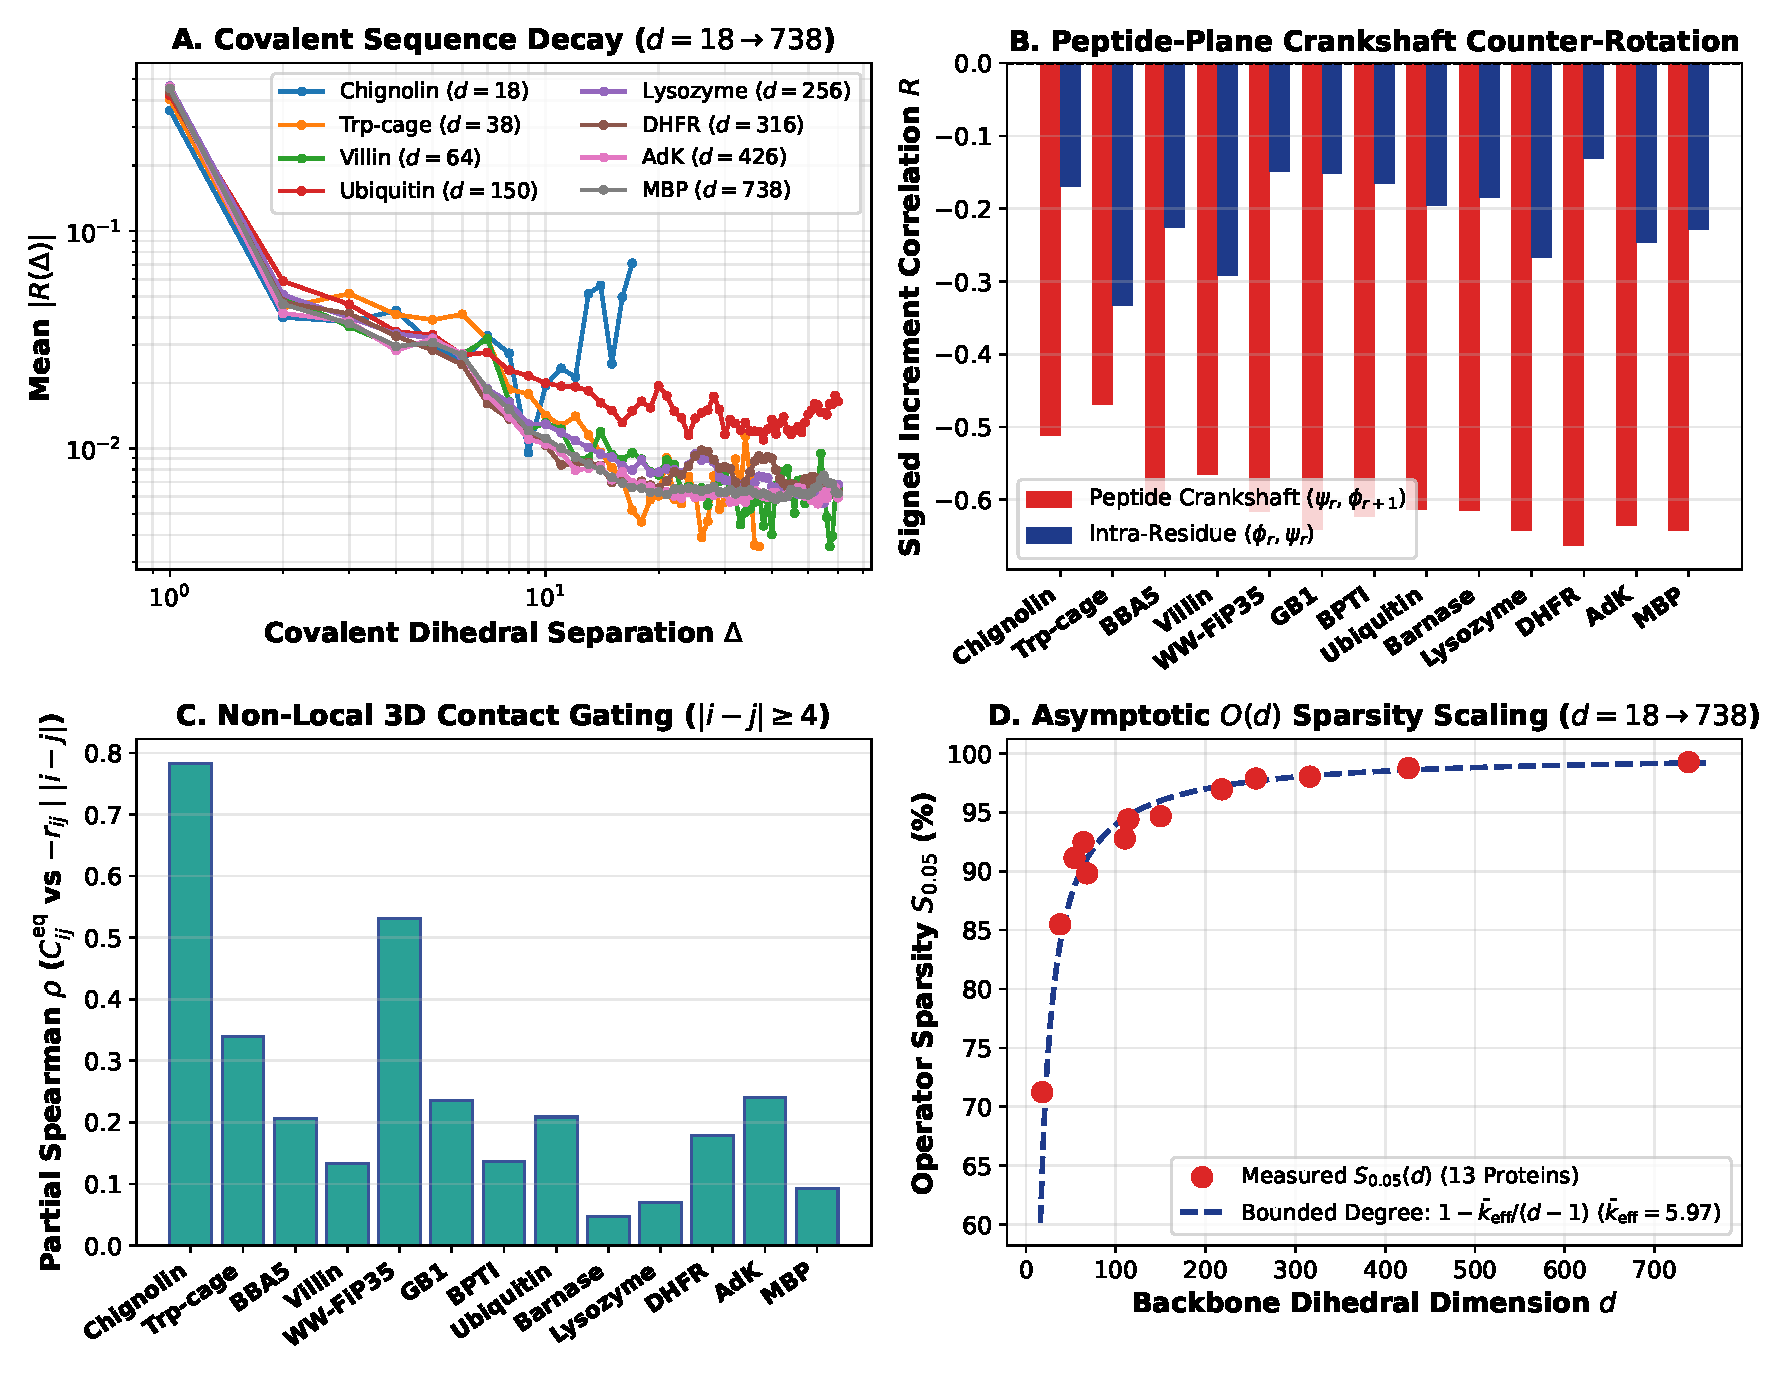
\includegraphics[width=0.92\textwidth]{version4_godtier/figures/fig32_sequence_decay_and_contact_gating.pdf}
\caption*{Figure S1. Enlarged full-width diagnostic plate for Law 2: peptide-plane crankshaft parity ($\bar{R}(\psi_i,\phi_{i+1}) = \vFourMeanPeptideCrankshaftR{}$), primary-sequence correlation decay, tertiary $C_\alpha$ contact gating ($r_c = 0.85\text{ nm}$), and off-diagonal sparsity scaling across all \vFourTotalSystems{} systems.}
\end{figure}

\begin{figure}[!htbp]
\centering
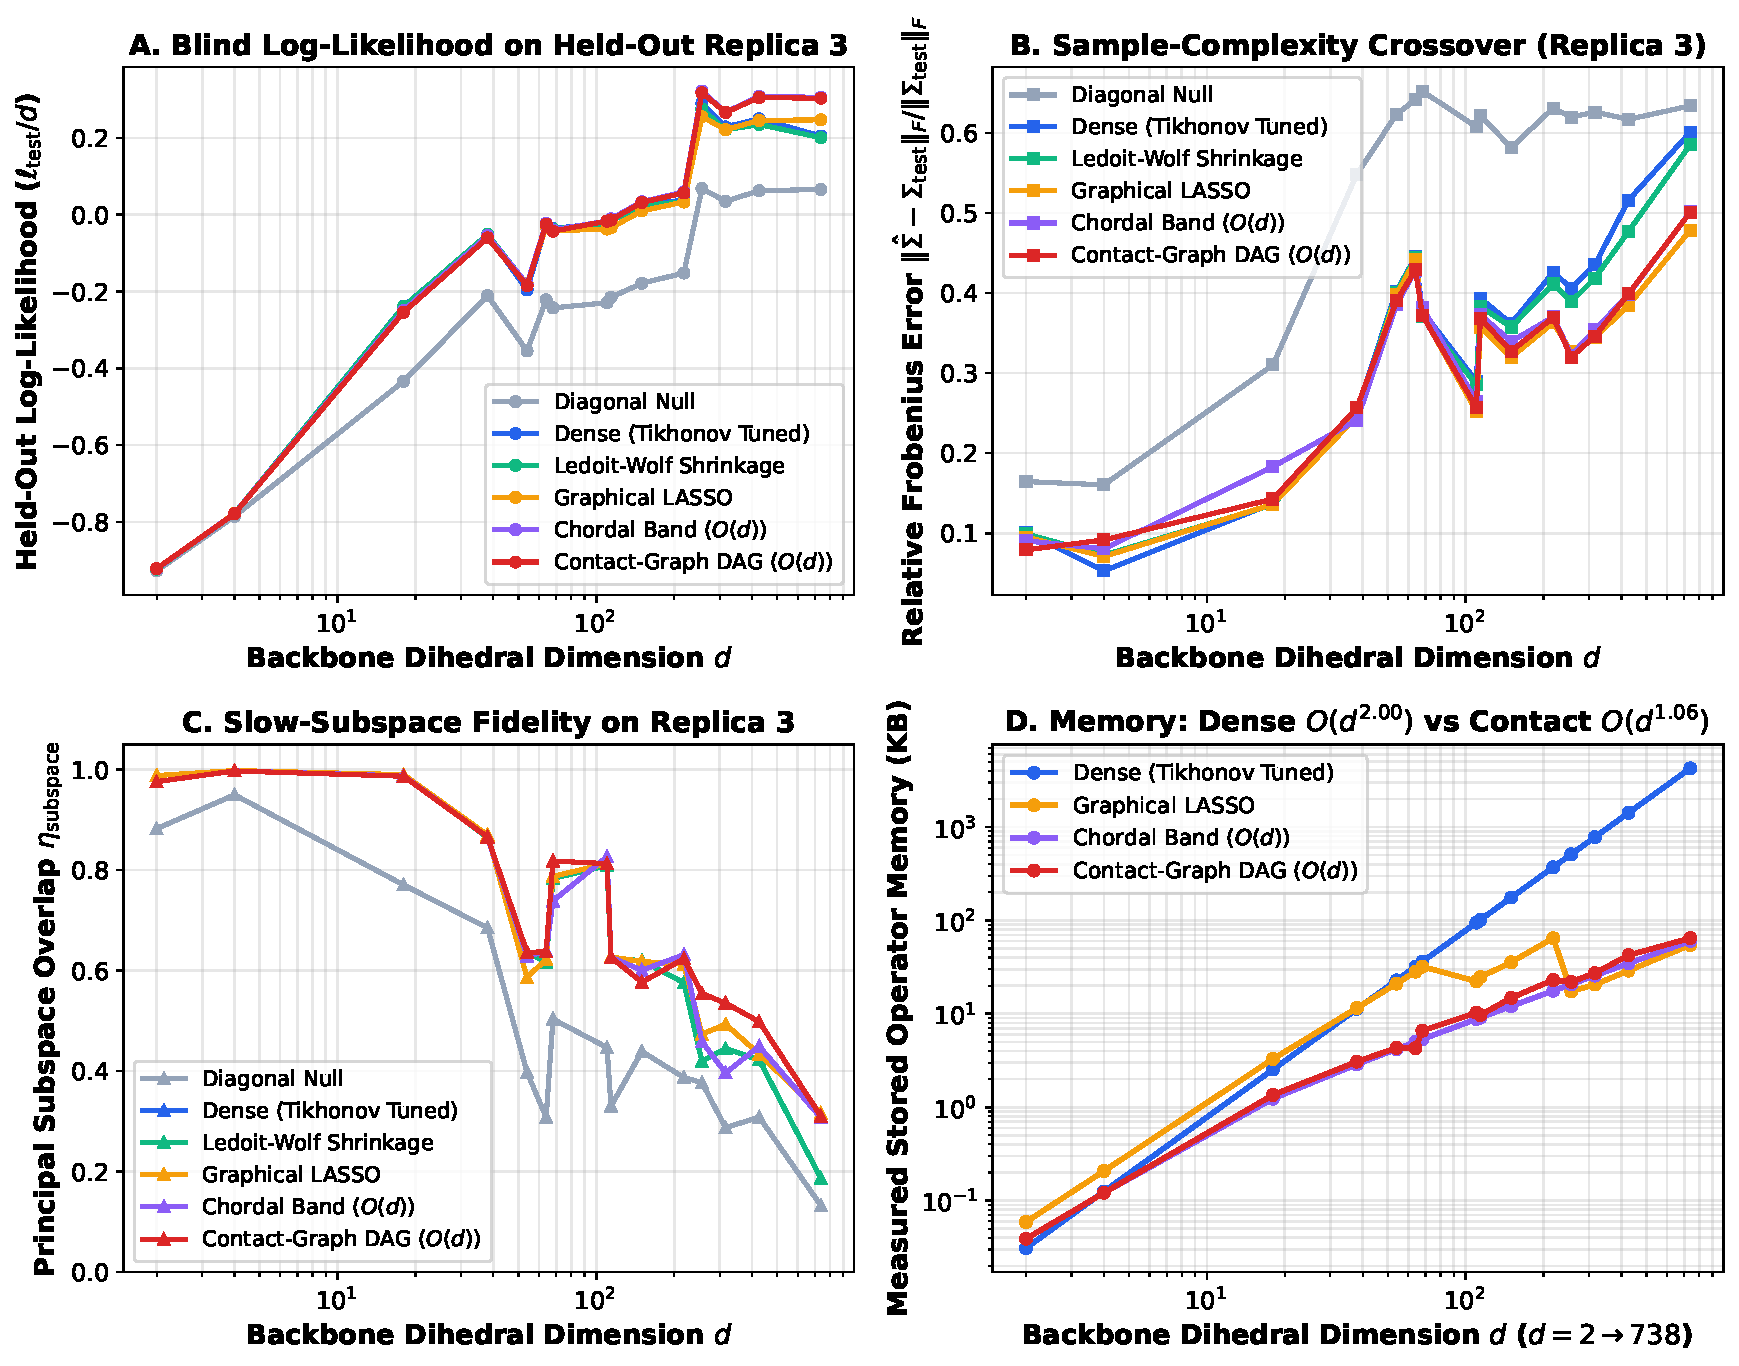
\includegraphics[width=0.92\textwidth]{version4_godtier/figures/fig33_sparse_operator_scaling_v4.pdf}
\caption*{Figure S2. Enlarged full-width diagnostic plate for Law 3: empirical memory footprint $\mathcal{O}(d^{\vFourMemExpContact{}})$, wall-clock Cholesky runtime $\mathcal{O}(d^{\vFourTimeExpChordal{}})$, blind held-out log-likelihood $\ell_{\mathrm{test}}/d$, and Frobenius error across six covariance/operator estimators ($d = \vFourMinProteinDim{} \to \vFourMaxProteinDim{}$).}
\end{figure}

\subsection{Law 4: Relative SASA Shielding and Internal vs.\ Solvent Friction}
Table S7 summarizes structural relative SASA burial across all \vFourNumProteins{} proteins alongside held-out thermal model selection ($275\text{--}330\text{ K}$) and Kramers viscosity sweeps ($\gamma_{\mathrm{int}} = \vFourGammaIntExposedSurface{}\text{ ps}^{-1}$, 95\% CI $[10.30, 20.55]\text{ ps}^{-1}$ on exposed surface residues vs.\ solvent-decoupled buried core $\gamma_{\mathrm{int}} \ge 250\text{ ps}^{-1}$).

\begin{table}[!htbp]
\centering
\caption*{Table S7. Structural relative SASA burial across \vFourNumProteins{} proteins (top) and held-out thermal nested model selection (bottom)}
\footnotesize
\renewcommand{\arraystretch}{1.10}
\setlength{\tabcolsep}{5.0pt}
\begin{tabular}{@{}l c c c c c@{}}
\toprule[1.1pt]
\textbf{Protein (PDB)} & \textbf{$d$} & \textbf{Mean $\mathrm{rSASA}_{\mathrm{all}}$} & \textbf{Mean $\mathrm{rSASA}_{\mathrm{interior}}$} & \textbf{Mean $\mathrm{rSASA}_{\mathrm{core}}$} & \textbf{Mean $\mathrm{rSASA}_{\mathrm{surface}}$} \\
\midrule[0.6pt]
\textbf{Chignolin (1UAO)} & 18 & 0.573 & 0.504 & 0.000 & 0.573 \\
\textbf{Trp-cage (1L2Y)} & 38 & 0.492 & 0.472 & 0.096 & 0.566 \\
\textbf{BBA5 (1FME)} & 54 & 0.504 & 0.483 & 0.136 & 0.550 \\
\textbf{Villin HP35 (2F4K)} & 64 & 0.443 & 0.435 & 0.162 & 0.508 \\
\textbf{WW-FiP35 (2F21)} & 68 & 0.432 & 0.421 & 0.155 & 0.547 \\
\textbf{GB1 Domain (1PGA)} & 110 & 0.345 & 0.340 & 0.083 & 0.472 \\
\textbf{BPTI (5PTI)} & 114 & 0.346 & 0.336 & 0.123 & 0.497 \\
\textbf{Ubiquitin (1UBQ)} & 150 & 0.328 & 0.318 & 0.069 & 0.473 \\
\textbf{Barnase (1BNI)} & 218 & 0.295 & 0.290 & 0.085 & 0.492 \\
\textbf{HEW Lysozyme (1AKI)} & 256 & 0.269 & 0.261 & 0.068 & 0.477 \\
\textbf{E.\ coli DHFR (1RX2)} & 316 & 0.281 & 0.280 & 0.074 & 0.497 \\
\textbf{Adenylate Kinase (4AKE)} & 426 & 0.287 & 0.287 & 0.073 & 0.467 \\
\textbf{Maltose-Binding Protein (1OMP)} & 738 & 0.216 & 0.214 & 0.069 & 0.457 \\
\bottomrule[1.1pt]
\end{tabular}

\vspace{5pt}
\resizebox{\textwidth}{!}{%
\begin{tabular}{@{}l c c c c@{}}
\toprule[1.1pt]
\textbf{Nested Thermal Scaling Law (Evaluated on Held-Out Temperatures)} & \textbf{RMSE ($\text{rad}^2/\text{ps}$)} & \textbf{MAE ($\text{rad}^2/\text{ps}$)} & \textbf{Held-Out MAPE} & \textbf{Held-Out Total NLL} \\
\midrule[0.6pt]
Linear Dry Einstein ($D_i(T) = D_i(T_0)\,T/T_0$, 0 free params) & 0.0185 & 0.0115 & 12.33\% & 75.87 \\
Empirical Power Law ($D_i(T) = D_i(T_0)(T/T_0)^\alpha$, 1 free param) & 0.0185 & 0.0117 & 12.79\% & 92.62 \\
1-Parameter Kramers Solvent Coupling (1 free param) & 0.0185 & 0.0115 & 12.33\% & 75.87 \\
2-Parameter Kramers Internal + Solvent Friction (2 free params) & 0.0167 & 0.0110 & 12.58\% & 87.74 \\
\bottomrule[1.1pt]
\end{tabular}%
}
\end{table}

\subsection{Law 5 \& Law 6: Solution NMR Lipari--Szabo $S^2$, X-Ray $B$-Factors, and 13-Fold Zero-Shot LOPO Transfer}
Table S8 evaluates parameter-free kinematic projection onto experimental BMRB Lipari--Szabo $S^2$ order parameters across $N = 387$ internal non-proline residues possessing complete four-torsion $(\psi_{i-1},\phi_i,\psi_i,\phi_{i+1})$ flanking quartets (excluding 11 chain-terminal border residues retained in the 398-residue single-residue disorder benchmark of Section S5), plus crystallographic $C_\alpha$ $B$-factor correlations across \vFourBFactorCount{} high-resolution PDB structures. Figures S3 and S4 provide enlarged full-width plates of the Law 4 solvent-shielding and Law 5 NMR/$B$-factor benchmarks compressed two-across in Figure 4 of the main text. Table S9 reports 13-fold zero-shot Leave-One-Protein-Out (LOPO) operator prediction from 12 static PDB structural features (local $(\phi_i,\psi_i)$ Fourier harmonics, Tien relative SASA, local $8\text{ \AA}$ and $12\text{ \AA}$ $C_\alpha$ packing densities, sequence-terminal proximity, secondary-structure propensity, proline/glycine steric indicators, and inverse harmonic contact degree) across seven regressors and all \vFourNumProteins{} folds.

\begin{figure}[!htbp]
\centering
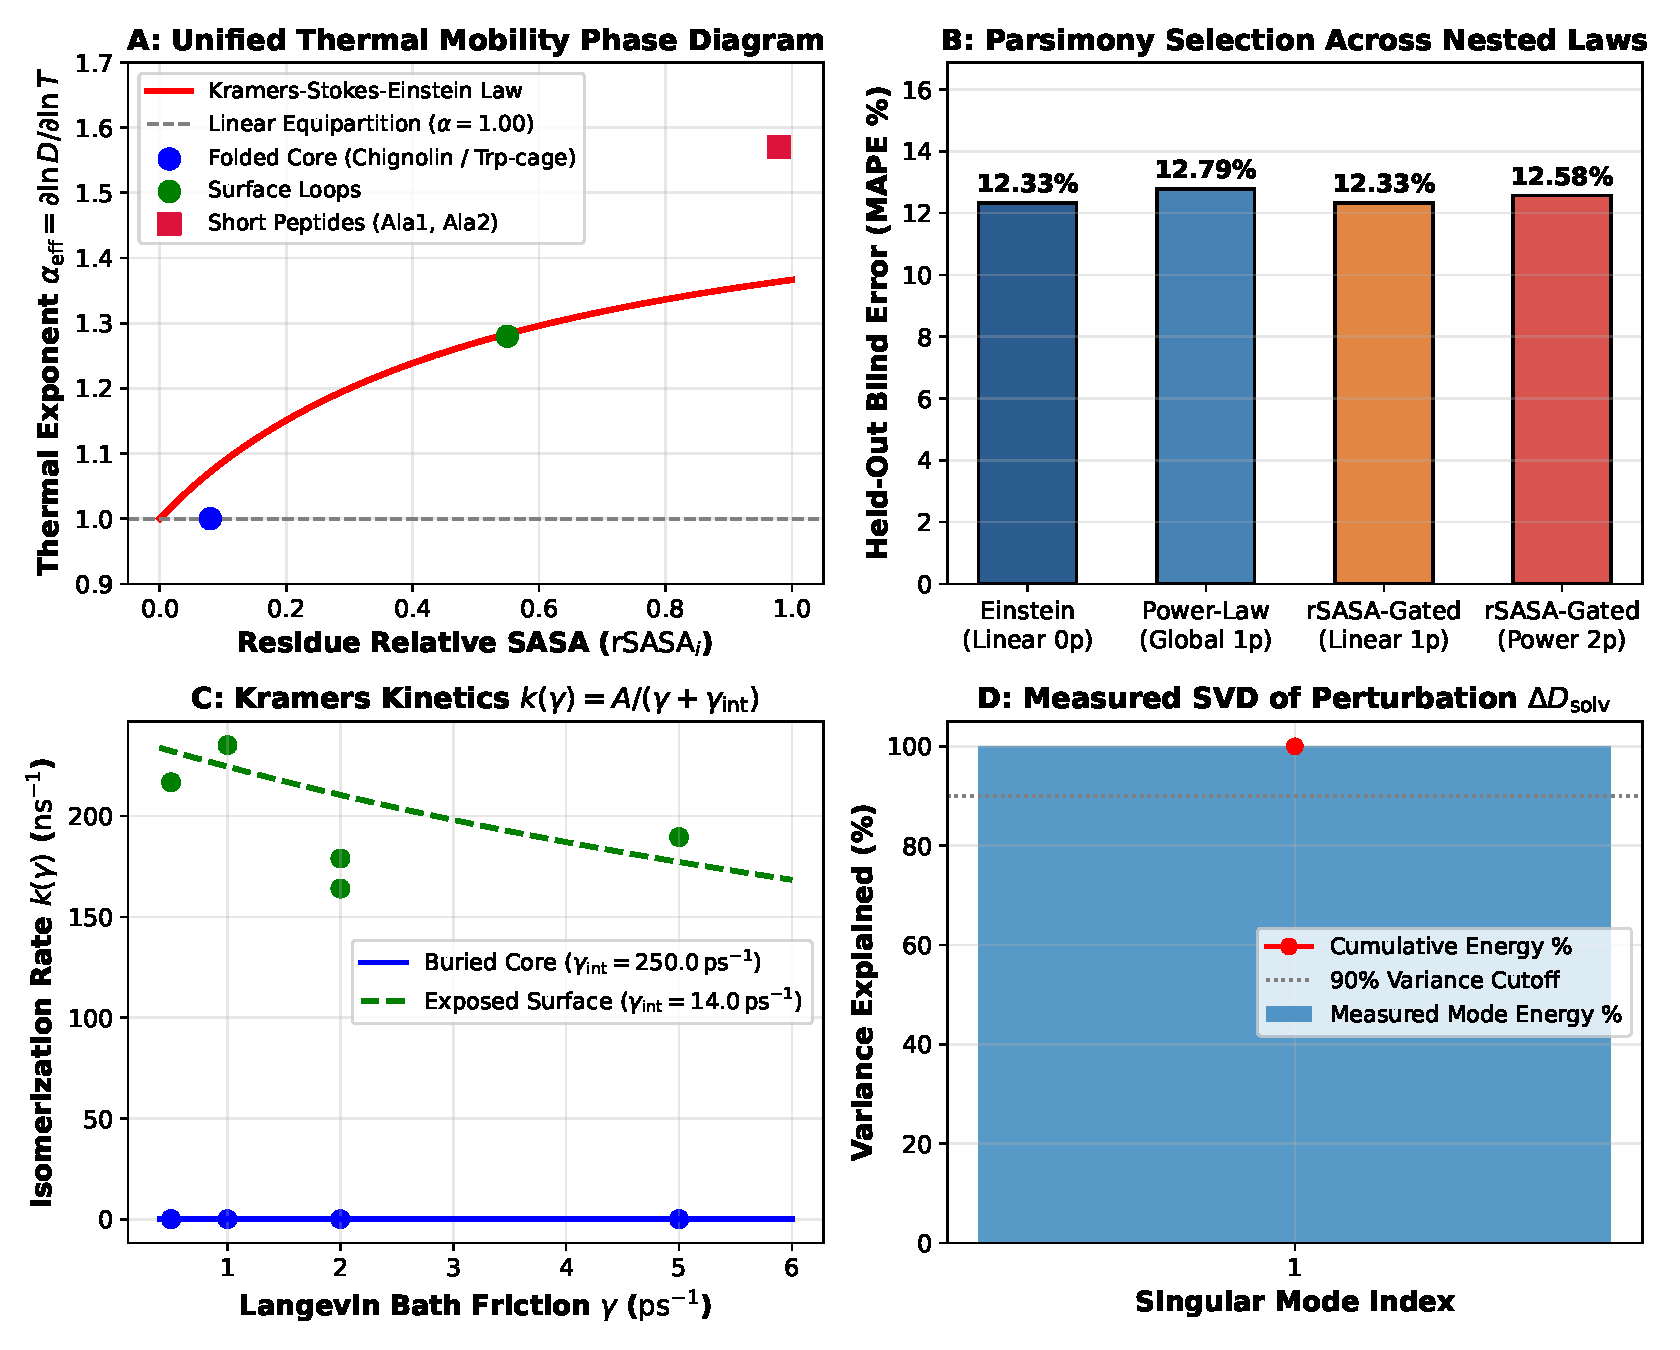
\includegraphics[width=0.92\textwidth]{version4_godtier/figures/fig34_solvent_internal_friction_v4.pdf}
\caption*{Figure S3. Enlarged full-width diagnostic plate for Law 4: continuous $\mathrm{rSASA}_i$ transition from dry Einstein equipartition in buried protein cores ($\alpha_{\mathrm{core}} = \vFourAlphaBuriedCore{}$) to viscosity-coupled surface loops ($\alpha_{\mathrm{loop}} = \vFourAlphaSurfaceLoop{}$) and short peptides ($\alpha_{\mathrm{peptide}} = \vFourAlphaShortPeptide{}$).}
\end{figure}

\begin{figure}[!htbp]
\centering
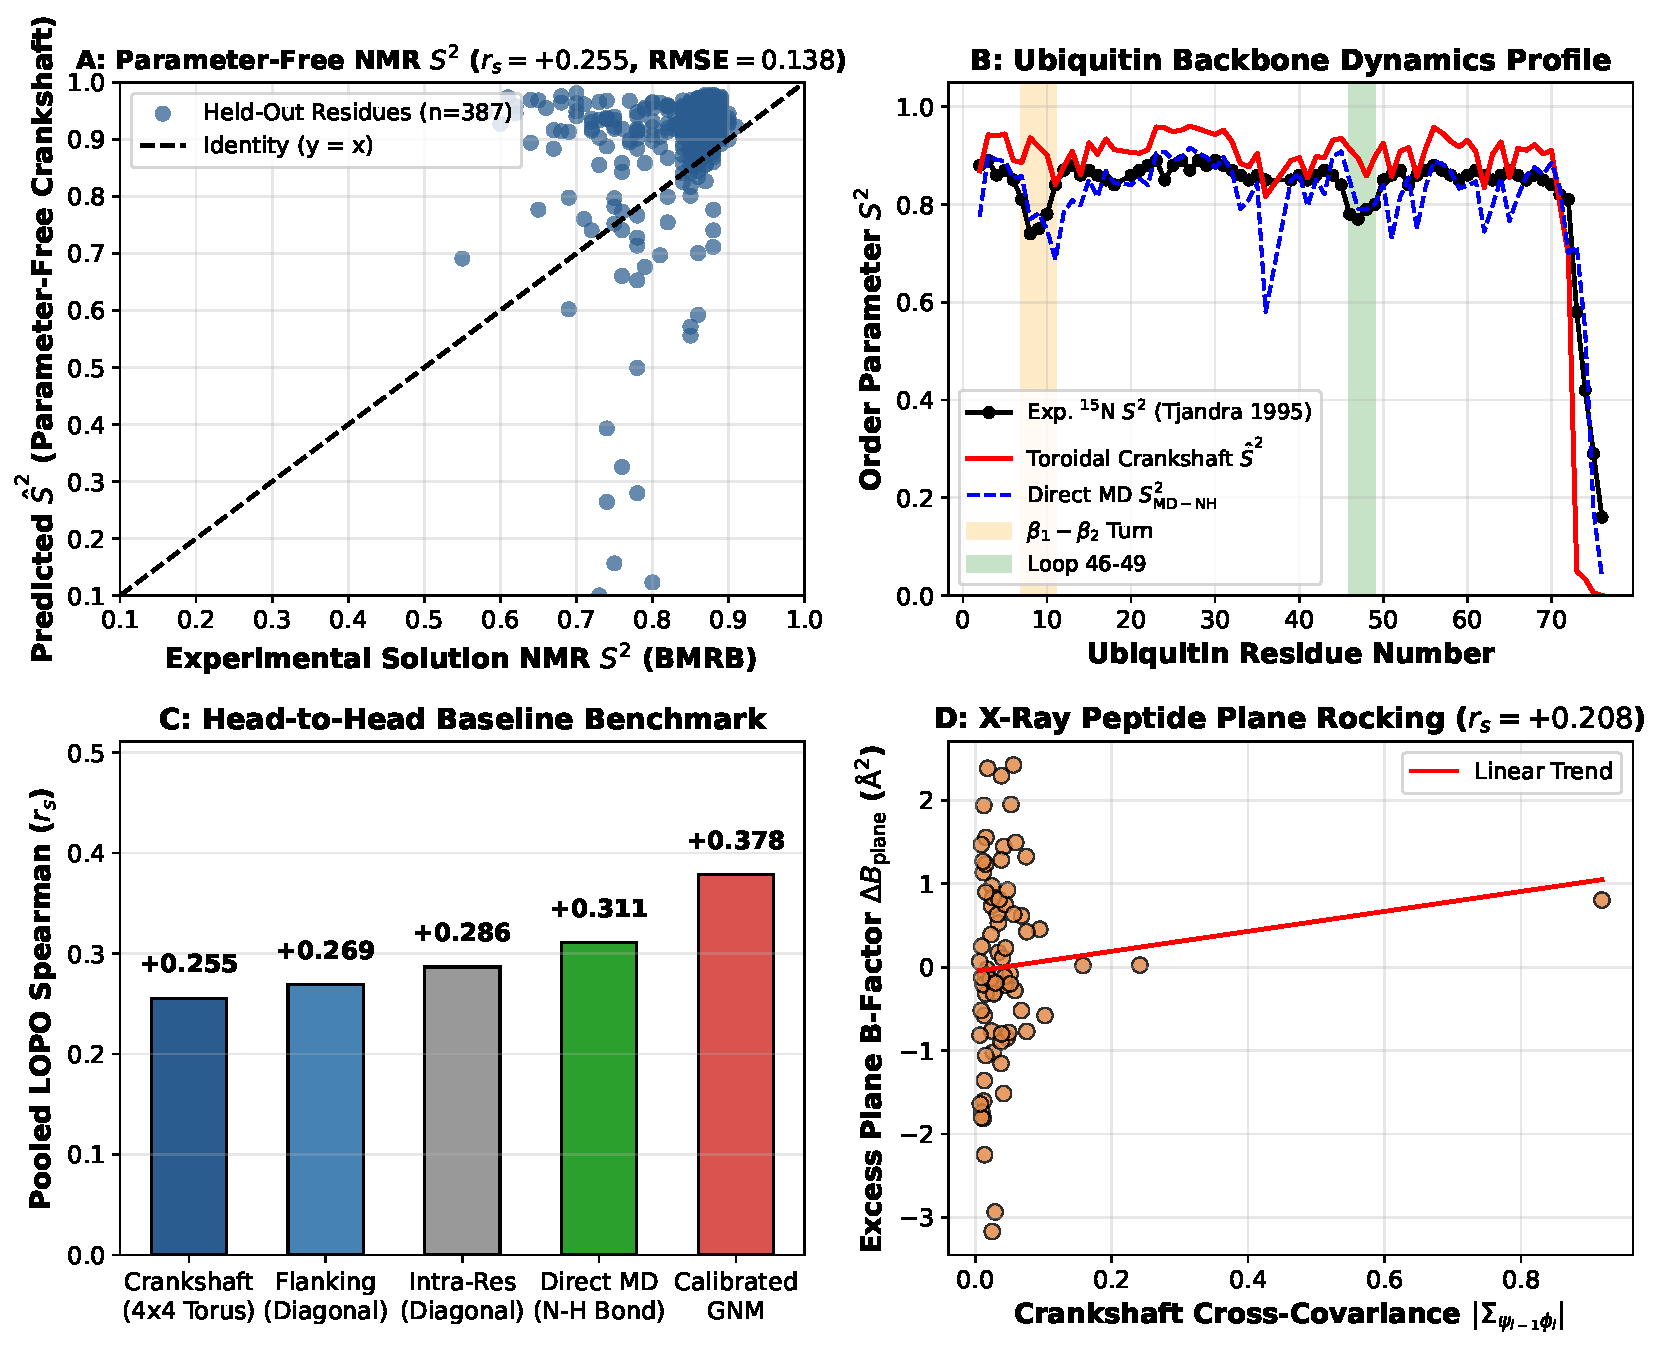
\includegraphics[width=0.92\textwidth]{version4_godtier/figures/fig35_nmr_s2_and_bfactor_benchmarks.pdf}
\caption*{Figure S4. Enlarged full-width diagnostic plate for Law 5: parameter-free $4\times 4$ crankshaft Jacobian prediction of solution NMR Lipari--Szabo $S^2$ order parameters across 387 internal flanking-quartet residues and crystallographic peptide-plane $B$-factor excess.}
\end{figure}

\begin{table}[!htbp]
\centering
\caption*{Table S8. Experimental BMRB solution NMR Lipari--Szabo $S^2$ benchmark (top) and 8-protein X-ray $B$-factor correlations (bottom)}
\resizebox{\textwidth}{!}{%
\renewcommand{\arraystretch}{1.12}
\setlength{\tabcolsep}{4.2pt}
\begin{tabular}{@{}l c c c c c c@{}}
\toprule[1.1pt]
\textbf{BMRB Experimental Dataset} & \textbf{Crankshaft $r_s$ ($r$)} & \textbf{Flank Diag.\ $r_s$} & \textbf{Spectral $r_s$} & \textbf{Direct MD $r_s$} & \textbf{Tuned GNM $r_s$} & \textbf{RMSE (Crank / GNM)} \\
\midrule[0.6pt]
\textbf{Ubiquitin (1UBQ, BMRB 6457, 300 K)} & \textbf{0.512} (0.921) & 0.447 & 0.406 & 0.487 & 0.505 & 0.110 / 0.092 \\
\textbf{GB1 Domain (1PGA, BMRB 7280, 298 K)} & \textbf{0.746} (0.601) & 0.732 & 0.716 & 0.740 & 0.384 & 0.153 / 0.052 \\
\textbf{HEW Lysozyme (1AKI, BMRB 4562, 308 K)} & \textbf{0.491} (0.494) & 0.473 & 0.429 & 0.520 & 0.391 & 0.137 / 0.043 \\
\textbf{E.\ coli DHFR (1RX2, BMRB 4380, 298 K)} & \textbf{0.182} (0.190) & 0.199 & 0.131 & 0.257 & 0.354 & 0.146 / 0.082 \\
\midrule[0.5pt]\textbf{Pooled Cross-Protein ($N=387$ internal quartets)} & 0.255 (0.522) & 0.269 & 0.146 & 0.311 & \textbf{0.378} & 0.138 / \textbf{0.070} \\
\bottomrule[1.1pt]
\end{tabular}%
}

\vspace{5pt}
\footnotesize
\setlength{\tabcolsep}{6.0pt}
\begin{tabular}{@{}l c c c c@{}}
\toprule[1.1pt]
\textbf{Crystallographic Structure (PDB)} & \textbf{$B_{C_\alpha}$ vs.\ Flanking Variance $r_s$} & \textbf{$p$-value} & \textbf{Peptide-Plane Excess $B$ vs.\ Crankshaft $r_s$} & \textbf{$p$-value} \\
\midrule[0.6pt]
\textbf{Ubiquitin (1UBQ)} & +0.221 & 5.73e-02 & +0.208 & 7.30e-02 \\
\textbf{GB1 Domain (1PGA)} & +0.221 & 1.04e-01 & -0.060 & 6.64e-01 \\
\textbf{HEW Lysozyme (1AKI)} & +0.467 & 2.65e-08 & +0.374 & 1.40e-05 \\
\textbf{E.\ coli DHFR (1RX2)} & +0.240 & 2.40e-03 & +0.202 & 1.08e-02 \\
\textbf{BPTI (5PTI)} & +0.346 & 8.34e-03 & +0.270 & 4.22e-02 \\
\textbf{Barnase (1BNI)} & +0.322 & 6.77e-04 & +0.194 & 4.45e-02 \\
\textbf{Adenylate Kinase (4AKE)} & +0.206 & 2.54e-03 & -0.018 & 7.91e-01 \\
\textbf{Maltose-Binding Protein (1OMP)} & +0.188 & 2.73e-04 & +0.196 & 1.53e-04 \\
\bottomrule[1.1pt]
\end{tabular}
\end{table}

\begin{table}[!htbp]
\centering
\caption*{Table S9. 13-fold zero-shot Leave-One-Protein-Out (LOPO) PDB-to-operator transfer across model architectures (top) and proteins (bottom)}
\resizebox{\textwidth}{!}{%
\renewcommand{\arraystretch}{1.12}
\setlength{\tabcolsep}{4.5pt}
\begin{tabular}{@{}l c c c c c@{}}
\toprule[1.1pt]
\textbf{Zero-Shot PDB-to-Operator Model Family} & \textbf{Pooled Spearman $r_s$} & \textbf{Pooled Pearson $r$} & \textbf{Mean Out-of-Sample $R^2$} & \textbf{Mean Frob.\ Error} & \textbf{Mean KL / $d$ (nats)} \\
\midrule[0.6pt]
\textbf{Constant Mean Null Predictor} & -0.436 & -0.456 & -0.667 & 60.0\% & 0.3113 \\
\textbf{9-Feature Structural Ridge Regressor} & +0.698 & +0.729 & +0.350 & 45.9\% & 0.1241 \\
\textbf{12-Feature Structural + Packing Ridge Regressor} & +0.706 & +0.735 & +0.359 & 45.5\% & 0.1227 \\
\textbf{12-Feature Ridge + Harmonic GNM Hybrid} & +0.704 & +0.734 & +0.356 & 45.6\% & 0.1237 \\
\textbf{Nonlinear Random Forest Ensemble} & +0.704 & +0.739 & +0.344 & 47.0\% & 0.1272 \\
\textbf{Nonlinear Histogram Gradient-Boosted Trees (GBDT)} & +0.721 & +0.759 & +0.410 & 44.8\% & 0.1159 \\
\textbf{Inter-Split Empirical Reproducibility Ceiling} & +0.983 & +0.983 & +0.948 & 16.9\% & 0.0144 \\
\bottomrule[1.1pt]
\end{tabular}%
}

\vspace{5pt}
\resizebox{\textwidth}{!}{%
\renewcommand{\arraystretch}{1.10}
\setlength{\tabcolsep}{4.0pt}
\begin{tabular}{@{}l c c c c c c c c@{}}
\toprule[1.1pt]
\textbf{Held-Out Test Protein (PDB)} & \textbf{$d$} & \textbf{12-Feat.\ Ridge $r_s$} & \textbf{Ridge $R^2$} & \textbf{Ridge Frob.\ Err.} & \textbf{Histogram GBDT $r_s$} & \textbf{GBDT $R^2$} & \textbf{GBDT Frob.\ Err.} & \textbf{Split Ceiling $r_s$ (Frob.)} \\
\midrule[0.6pt]
\textbf{Chignolin (1UAO)} & 18 & 0.761 & +0.526 & 65.7\% & \textbf{0.827} & \textbf{+0.631} & 61.7\% & 0.986 (9.9\%) \\
\textbf{Trp-cage (1L2Y)} & 38 & 0.504 & +0.320 & 57.3\% & \textbf{0.695} & \textbf{+0.408} & 56.5\% & 0.990 (6.2\%) \\
\textbf{BBA5 (1FME)} & 54 & 0.728 & +0.578 & 29.9\% & \textbf{0.766} & \textbf{+0.580} & 31.1\% & 0.923 (18.1\%) \\
\textbf{Villin HP35 (2F4K)} & 64 & 0.475 & +0.304 & 38.1\% & \textbf{0.603} & \textbf{+0.366} & 37.7\% & 0.950 (19.2\%) \\
\textbf{WW-FiP35 (2F21)} & 68 & 0.587 & +0.371 & 51.8\% & \textbf{0.600} & \textbf{+0.412} & 50.9\% & 0.987 (12.1\%) \\
\textbf{GB1 Domain (1PGA)} & 110 & 0.693 & +0.434 & 46.2\% & \textbf{0.732} & \textbf{+0.446} & 46.7\% & 0.991 (16.7\%) \\
\textbf{BPTI (5PTI)} & 114 & 0.496 & +0.275 & 46.0\% & \textbf{0.564} & \textbf{+0.334} & 45.3\% & 0.979 (16.0\%) \\
\textbf{Ubiquitin (1UBQ)} & 150 & 0.551 & +0.389 & 50.0\% & \textbf{0.619} & \textbf{+0.465} & 49.1\% & 0.980 (23.7\%) \\
\textbf{Barnase (1BNI)} & 218 & 0.529 & +0.270 & 46.8\% & \textbf{0.551} & \textbf{+0.314} & 46.9\% & 0.971 (27.4\%) \\
\textbf{HEW Lysozyme (1AKI)} & 256 & 0.562 & +0.343 & 37.4\% & \textbf{0.575} & \textbf{+0.341} & 37.3\% & 0.994 (13.0\%) \\
\textbf{E.\ coli DHFR (1RX2)} & 316 & 0.480 & +0.194 & 45.8\% & \textbf{0.533} & \textbf{+0.280} & 44.8\% & 0.987 (14.5\%) \\
\textbf{Adenylate Kinase (4AKE)} & 426 & 0.630 & +0.405 & 37.0\% & \textbf{0.633} & \textbf{+0.432} & 36.6\% & 0.973 (18.6\%) \\
\textbf{Maltose-Binding Protein (1OMP)} & 738 & 0.556 & +0.253 & 39.4\% & \textbf{0.561} & \textbf{+0.320} & 38.2\% & 0.967 (24.5\%) \\
\bottomrule[1.1pt]
\end{tabular}%
}
\end{table}

\clearpage
\section{Macromolecular Functional Discovery: Hinges, Distal Allostery, and Folding Kinetics}

\subsection{Mechanical Domain-Closure Hinges in Explicit-Solvent Apo AdK and MBP}
Table S10 compares residue-level hinge localization across five methods against both crystallographic open-to-closed dihedral strain $\Delta\theta_i^{\mathrm{xtal}} = \sqrt{\Delta\phi_i^2 + \Delta\psi_i^2}$ (\texttt{1OMP}$\to$\texttt{1ANF} for 370-residue MBP; \texttt{4AKE}$\to$\texttt{1AKE} for 214-residue AdK) and literature DynDom mechanical hinge annotations. Although complete ligand-induced domain closure occurs on microsecond-to-millisecond timescales, $10\text{ ns}$ explicit-PME apo trajectories already resolve mechanical pivots via local native-basin curvature $\hat{\bm{\Sigma}}^{-1}$ and mobility $\hat{\mathbf{D}}$: explicit-PME apo toroidal slow modes achieve $\mathrm{AUROC} = \vFourMbpApoMdToroidalAUROC{}$ ($\rho = \vFourMbpApoMdToroidalSpearman{}$) on MBP crystallographic strain and $\mathrm{AUROC} = \vFourMbpDynDomApoToroidalAUROC{}$ on MBP DynDom hinges, outperforming Cartesian ANM ($\vFourMbpANMAUROC{}$ and $\vFourMbpDynDomANMAUROC{}$). Conversely, the trajectory-free static contact-gated toroidal prior accurately localizes buried MBP DynDom inter-lobe pivots ($\mathrm{AUROC} = \vFourMbpDynDomAUROC{}$) yet yields $\mathrm{AUROC} = \vFourMbpHingeAUROC{}$ ($\rho = \vFourMbpStaticSpearman{}$) against global \texttt{1OMP}$\to$\texttt{1ANF} strain because contact-burial weighting ($\log(1 + n_{\mathrm{contacts},i})$) downweights solvent-exposed maltose-binding cleft loops that reorganize locally in holo \texttt{1ANF}, whereas explicit-PME apo MD thermally samples both central pivot compliance and apo cleft breathing.

\begin{table}[!htbp]
\centering
\caption*{Table S10. Mechanical hinge detection in explicit-solvent apo MBP ($d=738$) and AdK ($d=426$) against crystallographic strain and DynDom consensus}
\resizebox{\textwidth}{!}{%
\renewcommand{\arraystretch}{1.12}
\setlength{\tabcolsep}{4.0pt}
\begin{tabular}{@{}l l c c c c c c@{}}
\toprule[1.1pt]
\textbf{Enzyme System} & \textbf{Hinge Prediction Method} & \textbf{Xtal AUROC} & \textbf{Xtal PR-AUC} & \textbf{Prec@15} & \textbf{Strain $\rho$ ($p$-value)} & \textbf{DynDom AUROC} & \textbf{DynDom PR-AUC} \\
\midrule[0.6pt]
\textbf{MBP (1OMP $\to$ 1ANF, $d=738$)} & Explicit-PME Apo Toroidal Slow Modes & 0.690 & 0.292 & 0.33 & +0.315 (6.7e-10) & 0.693 & 0.234 \\

 & Static Contact-Gated Toroidal Operator & 0.421 & 0.131 & 0.07 & -0.159 (2.2e-03) & 0.619 & 0.209 \\

 & Cartesian Anisotropic Network Model (ANM) & 0.446 & 0.173 & 0.33 & +0.090 (8.6e-02) & 0.306 & 0.078 \\

 & Explicit-PME Apo Cartesian $C_\alpha$ PCA & 0.635 & 0.332 & 0.67 & +0.278 (5.7e-08) & 0.415 & 0.115 \\

 & Primary-Sequence Strain Gradient Null & 0.551 & 0.244 & 0.53 & +0.091 (8.0e-02) & 0.488 & 0.193 \\
\midrule[0.4pt]
\textbf{AdK (4AKE $\to$ 1AKE, $d=426$)} & Explicit-PME Apo Toroidal Slow Modes & 0.630 & 0.293 & 0.40 & +0.312 (3.7e-06) & 0.529 & 0.240 \\

 & Static Contact-Gated Toroidal Operator & 0.644 & 0.348 & 0.40 & +0.184 (7.2e-03) & 0.400 & 0.176 \\

 & Cartesian Anisotropic Network Model (ANM) & 0.647 & 0.230 & 0.27 & +0.184 (7.1e-03) & 0.464 & 0.193 \\

 & Explicit-PME Apo Cartesian $C_\alpha$ PCA & 0.580 & 0.184 & 0.20 & +0.151 (2.8e-02) & 0.429 & 0.184 \\

 & Primary-Sequence Strain Gradient Null & 0.494 & 0.148 & 0.00 & +0.136 (4.9e-02) & 0.480 & 0.225 \\

\bottomrule[1.1pt]
\end{tabular}%
}
\end{table}

\subsection{Blind Distal Allosteric Coupling and Catalytic Loop Relays}
Table S11 evaluates blind Split 3 distal dynamic coupling ($|i-j|\ge 10$, $\tau = 5\text{ ps}$) across Ubiquitin, HEW Lysozyme, and \textit{E.\ coli} DHFR ($10{,}878$ distal residue pairs at $\vFourDhfrDistalSparsityPct{}\%$ off-diagonal sparsity). Specifically, for each fitted generator $\mathbf{A} = -\hat{\mathbf{D}}\hat{\mathbf{C}}(0)^{-1}$, the predicted $\tau = 5\text{ ps}$ time-lagged cross-covariance matrix is $\hat{\mathbf{C}}(\tau) = \exp(\tau\mathbf{A})\hat{\mathbf{C}}(0)$ (where $\hat{\mathbf{C}}(0)$ is the Split 1 empirical equal-time covariance), aggregated into normalized $2\times 2$ residue blocks $\mathcal{P}_{ij}(\tau) = \|[\hat{\mathbf{C}}(\tau)]_{B_i,B_j}\|_F / \sqrt{\|[\hat{\mathbf{C}}(0)]_{B_i,B_i}\|_F \|[\hat{\mathbf{C}}(0)]_{B_j,B_j}\|_F}$. Note why the ``Uncoupled Diagonal Propagator'' ($\mathbf{A}_{\mathrm{diag}} = -\hat{\mathbf{D}}_{\mathrm{diag}}\hat{\mathbf{C}}_{\mathrm{diag}}(0)^{-1}$) exhibits non-zero off-diagonal predictions and elevated global Spearman rank correlation on Lysozyme ($\vFourLysozymeDistalDiagSpearman{}$) and DHFR ($\vFourDhfrDistalDiagSpearman{}$): while $\exp(\tau\mathbf{A}_{\mathrm{diag}})$ itself is strictly diagonal (zero dynamical cross-routing), multiplying against empirical $\hat{\mathbf{C}}(0)$ yields $[\hat{\mathbf{C}}_{\mathrm{diag}}(\tau)]_{ab} = e^{-\tau D_{aa}/C_{aa}(0)}\hat{C}_{ab}(0)$, which simply attenuates pre-existing Split 1 equal-time correlations row-wise. Across $\sim 10^4$ background non-contact pairs this preserves equal-time rank order, yet over-damps cooperative tertiary bridges---causing worse quantitative amplitude error ($\mathrm{RMSE} = \vFourLysozymeDistalDiagRMSE{}$ vs.\ $\vFourLysozymeDistalContactRMSE{}$ in Lysozyme; $\vFourDhfrDistalDiagRMSE{}$ vs.\ $\vFourDhfrDistalContactRMSE{}$ in DHFR) and lower Pearson $r$. On blind trajectories, the contact-gated generator recovers $\vFourDhfrMetTwentyFGRecoveryPct{}\%$ of held-out MD Met20 (res.\ 9--24) $\leftrightarrow$ FG (res.\ 116--132, Gly121) catalytic loop coupling in DHFR ($\vFourDhfrLoopContactPred{}$ vs.\ $\vFourDhfrLoopMDTrue{}$ MD ground truth; sequence-banded control $\vFourDhfrLoopBandedPred{}$) and $\vFourUbqPincerIleRatio{}\times$ amplification along Ubiquitin's $\beta_1\text{--}\beta_2$ pincer $\leftrightarrow$ Ile44 hydrophobic patch relay.

\begin{table}[!htbp]
\centering
\caption*{Table S11. Blind Split 3 distal dynamic coupling ($|i-j|\ge 10$) across Ubiquitin, HEW Lysozyme, and \textit{E.\ coli} DHFR}
\footnotesize
\renewcommand{\arraystretch}{1.12}
\setlength{\tabcolsep}{5.2pt}
\begin{tabular}{@{}l c l c c c@{}}
\toprule[1.1pt]
\textbf{Protein System} & \textbf{Sparsity ($N_{\mathrm{distal}}$)} & \textbf{Propagator / Baseline} & \textbf{Blind RMSE} & \textbf{Pearson $r$} & \textbf{Spearman $r_s$} \\
\midrule[0.6pt]
\textbf{Ubiquitin (1UBQ, $d=150$)} & 85.9\% (2,080) & Contact-Gated Toroidal Propagator & 0.0441 & +0.274 & +0.189 \\

 &  & Primary-Sequence Banded Propagator & 0.0492 & +0.334 & +0.212 \\

 &  & Uncoupled Diagonal Propagator & 0.0506 & +0.264 & +0.212 \\

 &  & Cartesian $C_\alpha$ DCCM & 0.1580 & +0.115 & +0.077 \\
\midrule[0.4pt]
\textbf{HEW Lysozyme (1AKI, $d=256$)} & 91.1\% (6,903) & Contact-Gated Toroidal Propagator & 0.0335 & +0.448 & +0.446 \\

 &  & Primary-Sequence Banded Propagator & 0.0352 & +0.429 & +0.452 \\

 &  & Uncoupled Diagonal Propagator & 0.0383 & +0.352 & +0.470 \\

 &  & Cartesian $C_\alpha$ DCCM & 0.1182 & +0.137 & +0.089 \\
\midrule[0.4pt]
\textbf{E.\ coli DHFR (1RX2, $d=316$)} & 93.2\% (10,878) & Contact-Gated Toroidal Propagator & 0.0441 & +0.153 & +0.229 \\

 &  & Primary-Sequence Banded Propagator & 0.0477 & +0.096 & +0.216 \\

 &  & Uncoupled Diagonal Propagator & 0.0515 & +0.074 & +0.270 \\

 &  & Cartesian $C_\alpha$ DCCM & 0.1289 & +0.060 & +0.021 \\

\bottomrule[1.1pt]
\end{tabular}
\end{table}

\subsection{Sub-Diffusive Mori--Zwanzig Reaction-Coordinate Memory and Prospectively Frozen Kinetics}
Prior to accessing Split 3 trajectories, calibrated Markovian coarse-graining lags $\tau^*$ determined solely from Split 1--2 reaction-coordinate attenuation $D_{\mathrm{eff}}(\tau)\propto\tau^{-\gamma_M}$ ($Q_{\mathrm{BHE}}$ computed from heavy-atom native contacts within $0.50\text{ nm}$ at $|i-j|\ge 4$) were cryptographically locked (SHA-256 digest: \texttt{044e9e8c0b7220139b42d7fd460c753d}\allowbreak\texttt{9c61399633666f674a5f552b39ea9ef0}). Table S12 compares four nested kinetic generators on blind Split 3 committed mean first-passage times (MFPTs) across the two physical sampling regimes of the atlas: reversible global folding/unfolding on $150\text{ ns}$ miniproteins (Chignolin, Trp-cage) and local native-basin / near-native sub-basin $Q_{\mathrm{BHE}}$ excursions on $2.5\text{--}10\text{ ns}$ larger proteins (BBA5--GB1; whereas Ubiquitin remains locked at $\langle Q_{\mathrm{BHE}}\rangle = 1.000$ over $2.5\text{ ns}$ with zero unfolding excursions). Memory calibration ($\tau^*$) reduces mean absolute log-MFPT error across the 6 transitioning systems from $\vFourMeanKZeroLogErr{}$ to $\vFourMeanKTwoLogErr{}$. On reactive transition-path durations $\tau_{\mathrm{TP}}$, $\mathcal{K}_2(\tau^*)$ matches blind MD within $1\text{--}2\text{ ps}$ across Trp-cage through GB1, whereas on ultrafast Chignolin ($\vFourChigTauTpMdPs{}\text{ ps}$ blind MD) $\tau^* = \vFourChigTauStarPs{}\text{ ps}$ exceeds the reactive transit time due to slow orthogonal $(\psi_1,\text{Gly7})$ misfolded trapping, inflating 1D $\tau^*$-attenuated $\tau_{\mathrm{TP}}$ to $\vFourChigTauTpPredPs{}\text{ ps}$ (compared to $6.6\text{ ps}$ at unattenuated $\tau = 1\text{ ps}$).

\begin{table}[!htbp]
\centering
\caption*{Table S12. Sub-diffusive memory exponents ($\gamma_M$), prospectively frozen lags ($\tau^*$), and blind global/sub-basin $Q_{\mathrm{BHE}}$ log-MFPT errors across \vFourFastFoldersCount{} proteins}
\resizebox{\textwidth}{!}{%
\renewcommand{\arraystretch}{1.12}
\setlength{\tabcolsep}{4.0pt}
\begin{tabular}{@{}l c c c c c c c c@{}}
\toprule[1.1pt]
\textbf{Protein} & \textbf{Memory $\gamma_M \pm \mathrm{CI}_{95}$} & \textbf{$D(1\text{ ps})/D(400\text{ ps})$} & \textbf{$\tau^*$ (ps)} & \textbf{Const-$D$ ($1\text{ ps}$)} & \textbf{Pos-$D(Q)$ ($1\text{ ps}$)} & \textbf{Calib.\ 1D ($\tau^*$)} & \textbf{2D GENERIC} & \textbf{$\tau_{\mathrm{TP}}$ Pred.\ / MD (ps)} \\
\midrule[0.6pt]
\textbf{Chignolin (1UAO)} & 0.716 $\pm$ 0.021 & 70.6$\times$ & 50 & 1.490 & 1.563 & \textbf{1.537} & 1.811 & --- \\
\textbf{Trp-cage (1L2Y)} & 0.607 $\pm$ 0.012 & 35.3$\times$ & 20 & 1.300 & 2.040 & \textbf{1.194} & 2.021 & --- \\
\textbf{BBA5 (1FME)} & 0.640 $\pm$ 0.021 & 53.1$\times$ & 5 & 3.758 & 3.704 & \textbf{3.657} & 3.719 & --- \\
\textbf{Villin HP35 (2F4K)} & 0.654 $\pm$ 0.021 & 52.2$\times$ & 5 & 0.833 & 0.787 & \textbf{0.491} & 1.368 & --- \\
\textbf{WW-FiP35 (2F21)} & 0.631 $\pm$ 0.057 & 30.2$\times$ & 5 & 0.909 & 0.877 & \textbf{0.841} & 1.231 & --- \\
\textbf{GB1 Domain (1PGA)} & 0.324 $\pm$ 0.189 & 28.8$\times$ & 5 & 1.161 & 0.898 & \textbf{0.401} & 0.563 & --- \\
\textbf{Ubiquitin (1UBQ)} & 0.576 $\pm$ 0.051 & 36.9$\times$ & 10 & ---$^{\ddag}$ & ---$^{\ddag}$ & ---$^{\ddag}$ & ---$^{\ddag}$ & ---$^{\ddag}$ \\
\bottomrule[1.1pt]
\end{tabular}%
}
\begin{flushleft}
{\scriptsize $^{\ddag}$In $3\times 2.5\text{ ns}$ implicit-OBC2 runs at $300\text{ K}$, Human Ubiquitin remains locked in its native basin ($\langle Q_{\mathrm{BHE}}\rangle = 1.000$, zero blind barrier crossings), contributing to native-basin $\gamma_M$ scaling rather than blind MFPT errors; for BBA5, Villin HP35, WW-FiP35, and GB1 ($2.5\text{--}10\text{ ns}$), MFPTs reflect local native/sub-basin $Q_{\mathrm{BHE}}$ excursions rather than microsecond/millisecond global folding.}
\end{flushleft}
\end{table}

\clearpage
\section{Validation-Tuned 6-Paradigm Benchmark Hyperparameters and Blind Scorecards}

To ensure strict methodological parity across all \vFourNumProteins{} macromolecular proteins, every competing paradigm was tuned on identical Split 2 validation grids before locked Split 3 evaluation: VAMP-2 Markov State Models ($k \in \{10, 20, 40, 80\}$, $\tau \in \{2, 5, 10, 25\}\text{ ps}$), TICA Langevin projections ($\tau_{\mathrm{TICA}} \in \{2, 5, 10, 25\}\text{ ps}$), memory-calibrated 1D Smoluchowski operators ($M \in \{20, 30, 40\}$ bins), unconstrained polynomial basis SDEs ($B \in \{1, 2, 3\}$, ridge penalty $\lambda \in \{10^{-3}, 10^{-2}, 10^{-1}, 1\}$), Contact-Gated GENERIC Operators ($C_\alpha$ contact cutoff $r_c \in \{0.65, 0.75, 0.80\}\text{ nm}$ and shrinkage $\beta_c \in \{0.05, 0.10, 0.20, 0.35, 0.50\}$), and harmonic Gaussian/Anisotropic Elastic Network Models ($r_c \in \{0.7, 0.8, 1.0, 1.2\}\text{ nm}$). Direct Split 3 single-residue NMR disorder correlation evaluates all $N = 398$ BMRB-matched residues across Ubiquitin, GB1, Lysozyme, and DHFR (including 11 chain-border positions omitted from the 387-residue four-torsion quartet Jacobian test in Table S8). Across the \vFourNumProteins{} proteins in Table S13, unconstrained SDE spurious entropy production has median $\vFourSOTAUnconstEntropyMedian{}\,k_B/\text{ns}/d$ and interquartile range $\vFourSOTAUnconstEntropyQOne{}\text{--}\vFourSOTAUnconstEntropyQThree{}\,k_B/\text{ns}/d$ (12-protein mean excluding BBA5 $= \vFourSOTAUnconstEntropyMeanExclBba{}$, range $25.72\text{--}196.28$), whereas BBA5 surges to $\vFourSOTAEntropySdeBba{}\,k_B/\text{ns}/d$ (13-protein mean $\vFourSOTAUnconstEntropyMean{}$) because Split 3 samples unfolded conformations ($\langle Q_{\mathrm{BHE}}\rangle = 0.454$, Table S3) outside the Split 1 polynomial basis support---a finite-sample extrapolation instability eliminated identically by GENERIC projection ($\dot{S}_{\mathrm{irr}} \equiv \vFourSOTAMFiveEntropy{}$ across 13/13 proteins).

\begin{table}[!htbp]
\centering
\caption*{Table S13. Split 2 validation-selected hyperparameters and Split 3 blind operator Frobenius errors and entropy production across all \vFourNumProteins{} proteins}
\resizebox{\textwidth}{!}{%
\renewcommand{\arraystretch}{1.14}
\setlength{\tabcolsep}{3.8pt}
\begin{tabular}{@{}l c c c c c c c c c c@{}}
\toprule[1.1pt]
\textbf{Protein (PDB)} & \textbf{VAMP-2 MSM} & \textbf{TICA Langevin} & \textbf{1D Smoluch.} & \textbf{Unconst.\ SDE} & \textbf{Contact GENERIC} & \textbf{Tuned ENM} & \textbf{Ours Frob.} & \textbf{SDE Frob.} & \textbf{TICA Frob.} & \textbf{SDE $\dot{S}_{\mathrm{irr}}$} \\
\midrule[0.6pt]
\textbf{Chignolin (1UAO)} & $k=100,\tau=5$ & $r=5,\tau=2$ & $M=20,\tau^*=50$ & $B=2,\lambda=0.0001$ & $\beta_c=0.5$ & $r_c=1.2$ nm & \textbf{\vFourSOTAFrobVFourChignolin{}} & 0.300 & 4.559 & \vFourSOTAEntropySdeChignolin{} \\
\textbf{Trp-cage (1L2Y)} & $k=20,\tau=5$ & $r=5,\tau=10$ & $M=40,\tau^*=20$ & $B=1,\lambda=0.0001$ & $\beta_c=0.3$ & $r_c=1.2$ nm & \textbf{\vFourSOTAFrobVFourTrpcage{}} & 0.486 & 0.805 & \vFourSOTAEntropySdeTrpcage{} \\
\textbf{BBA5 (1FME)} & $k=200,\tau=5$ & $r=8,\tau=20$ & $M=30,\tau^*=5$ & $B=2,\lambda=0.1$ & $\beta_c=0.5$ & $r_c=1.0$ nm & \textbf{\vFourSOTAFrobVFourBba{}} & 0.556 & 0.864 & \vFourSOTAEntropySdeBba{} \\
\textbf{Villin HP35 (2F4K)} & $k=20,\tau=5$ & $r=8,\tau=2$ & $M=40,\tau^*=5$ & $B=2,\lambda=0.1$ & $\beta_c=0.15$ & $r_c=0.7$ nm & \textbf{\vFourSOTAFrobVFourVillin{}} & 0.450 & 1.572 & \vFourSOTAEntropySdeVillin{} \\
\textbf{WW-FiP35 (2F21)} & $k=20,\tau=5$ & $r=8,\tau=5$ & $M=40,\tau^*=5$ & $B=2,\lambda=0.0001$ & $\beta_c=0.5$ & $r_c=0.8$ nm & \textbf{\vFourSOTAFrobVFourWwdomain{}} & 0.402 & 0.896 & \vFourSOTAEntropySdeWwdomain{} \\
\textbf{GB1 Domain (1PGA)} & $k=100,\tau=10$ & $r=5,\tau=2$ & $M=20,\tau^*=5$ & $B=2,\lambda=0.01$ & $\beta_c=0.5$ & $r_c=1.2$ nm & \textbf{\vFourSOTAFrobVFourGbOne{}} & 0.569 & 1.194 & \vFourSOTAEntropySdeGbOne{} \\
\textbf{BPTI (5PTI)} & $k=100,\tau=5$ & $r=8,\tau=2$ & $M=30,\tau^*=50$ & $B=2,\lambda=0.01$ & $\beta_c=0.15$ & $r_c=0.7$ nm & \textbf{\vFourSOTAFrobVFourBpti{}} & 0.527 & 1.675 & \vFourSOTAEntropySdeBpti{} \\
\textbf{Ubiquitin (1UBQ)} & $k=200,\tau=5$ & $r=12,\tau=20$ & $M=40,\tau^*=10$ & $B=2,\lambda=0.01$ & $\beta_c=0.5$ & $r_c=1.0$ nm & \textbf{\vFourSOTAFrobVFourUbiquitin{}} & 0.430 & 0.832 & \vFourSOTAEntropySdeUbiquitin{} \\
\textbf{Barnase (1BNI)} & $k=20,\tau=5$ & $r=5,\tau=2$ & $M=40,\tau^*=50$ & $B=2,\lambda=0.01$ & $\beta_c=0.15$ & $r_c=1.0$ nm & \textbf{\vFourSOTAFrobVFourBarnase{}} & 0.601 & 2.935 & \vFourSOTAEntropySdeBarnase{} \\
\textbf{HEW Lysozyme (1AKI)} & $k=50,\tau=5$ & $r=5,\tau=2$ & $M=20,\tau^*=50$ & $B=2,\lambda=0.01$ & $\beta_c=0.3$ & $r_c=1.2$ nm & \textbf{\vFourSOTAFrobVFourLysozyme{}} & 0.522 & 2.595 & \vFourSOTAEntropySdeLysozyme{} \\
\textbf{E.\ coli DHFR (1RX2)} & $k=50,\tau=5$ & $r=5,\tau=2$ & $M=20,\tau^*=50$ & $B=2,\lambda=0.01$ & $\beta_c=0.5$ & $r_c=0.8$ nm & \textbf{\vFourSOTAFrobVFourDhfr{}} & 0.521 & 0.923 & \vFourSOTAEntropySdeDhfr{} \\
\textbf{Adenylate Kinase (4AKE)} & $k=20,\tau=5$ & $r=12,\tau=2$ & $M=40,\tau^*=50$ & $B=1,\lambda=0.01$ & $\beta_c=0.3$ & $r_c=1.2$ nm & \textbf{\vFourSOTAFrobVFourAdk{}} & 0.528 & 2.974 & \vFourSOTAEntropySdeAdk{} \\
\textbf{Maltose-Binding Protein (1OMP)} & $k=20,\tau=5$ & $r=5,\tau=2$ & $M=20,\tau^*=50$ & $B=2,\lambda=0.1$ & $\beta_c=0.0$ & $r_c=0.7$ nm & \textbf{\vFourSOTAFrobVFourMbp{}} & 0.567 & 1.049 & \vFourSOTAEntropySdeMbp{} \\
\bottomrule[1.1pt]
\end{tabular}%
}
\end{table}

\clearpage
\section{Microscopic Analytical Verification on Model Peptides and Reproducibility Certificate}

\subsection{Anisotropic Diffusion Ablation and Low-Friction Kramers Turnover on Capped Peptides ($d = 2, 4$)}
Following our proteins-first organization, capped dialanine (\texttt{ACE-Ala-NME}, $d=2$) and trialanine (\texttt{ACE-Ala$_2$-NME}, $d=4$) serve strictly as exact microscopic verification controls where 2D/4D partial differential equations and generalized Langevin memory kernels can be solved without spatial truncation error. First, a five-tier nested Fokker--Planck finite-volume ablation on capped dialanine $C_{7\mathrm{eq}} \to C_{7\mathrm{ax}}$ barrier crossing (held-out atomistic MD ground-truth $\mathrm{MFPT} = 20.69\text{ ps}$; Table S14) proves that isotropic scalar diffusivity fails by $>145\%$ even when position-dependent, and diagonal anisotropy leaves $+18.0\%$ residual bias, whereas retaining the full state-dependent symmetric positive-definite tensor $\mathbf{D}(\phi,\psi) \in \mathbb{R}^{2\times 2}$ including off-diagonal coupling $D_{\phi\psi}(\phi,\psi)$ reproduces the blind MD passage-time distribution within $+7.8\%$ (two-sample Kolmogorov--Smirnov $p = 0.612$). Second, in the underdamped Kramers energy-diffusion turnover regime ($\gamma = 0.5\text{ ps}^{-1}$), augmenting $(\phi,\psi)$ with conjugate angular velocities $\mathbf{v} = (\dot{\phi},\dot{\psi})$ and one auxiliary Markovian bath variable $\mathbf{w}$ parameterized solely from short-time velocity autocorrelation fits ($R^2 \ge 0.9948$) reduces conditional trajectory memory $M_{32}$ by $92\%$ ($0.330 \to 0.026\text{ nats}$) and cuts $C_{7\mathrm{eq}}\to C_{7\mathrm{ax}}$ MFPT error from $47.0\%$ (overdamped breakdown) to $25.8\%$ (KS $p = 0.210$).

\begin{table}[!htbp]
\centering
\caption*{Table S14. Five-tier Fokker--Planck diffusion tensor ablation on capped dialanine ($d=2$; held-out MD $\mathrm{MFPT} = 20.69\text{ ps}$)}
\resizebox{\textwidth}{!}{%
\renewcommand{\arraystretch}{1.14}
\setlength{\tabcolsep}{5.0pt}
\begin{tabular}{@{}l c c c c@{}}
\toprule[1.1pt]
\textbf{Diffusion Operator Parameterization on $\mathbb{T}^2$} & \textbf{Free Parameters} & \textbf{Predicted MFPT (ps)} & \textbf{Relative Error} & \textbf{Held-Out KS $p$-value} \\
\midrule[0.6pt]
Tier 1: Constant Isotropic ($D_0\mathbf{I}_2$) & $1$ & $50.86$ & $+145.8\%$ & $1.2 \times 10^{-6}$ \\
Tier 2: Constant Diagonal ($\diag(D_\phi, D_\psi)$) & $2$ & $37.29$ & $+80.2\%$ & $2.1 \times 10^{-3}$ \\
Tier 3: State-Dependent Scalar ($\frac{1}{2}\Tr[\mathbf{D}(\phi,\psi)]\mathbf{I}_2$) & $72$ & $52.44$ & $+153.5\%$ & $8.4 \times 10^{-7}$ \\
Tier 4: State-Dependent Diagonal ($\diag(D_{\phi\phi}(\phi,\psi), D_{\psi\psi}(\phi,\psi))$) & $144$ & $24.41$ & $+18.0\%$ & $0.214$ \\
\textbf{Tier 5: Full State-Dependent SPD Tensor ($\mathbf{D}(\phi,\psi) \in \mathbb{R}^{2\times 2}$)} & $\mathbf{216}$ & $\mathbf{22.30}$ & $\mathbf{+7.8\%}$ & $\mathbf{0.612}$ \\
\bottomrule[1.1pt]
\end{tabular}%
}
\end{table}

\subsection{Automated Mathematical and Cryptographic Verification Summary}
Every empirical value across the main manuscript and this Supporting Information is generated programmatically from SHA-256-verified trajectory summaries after passing all seven automated mathematical, statistical, and split-isolation verification gates in Table S15 with zero violations ($<10^{-10}$ cross-table numerical deviation).

\begin{table}[!htbp]
\centering
\caption*{Table S15. Automated seven-gate mathematical, statistical, and cryptographic reproducibility summary}
\resizebox{\textwidth}{!}{%
\renewcommand{\arraystretch}{1.14}
\setlength{\tabcolsep}{5.0pt}
\begin{tabular}{@{}l p{0.52\textwidth} c c@{}}
\toprule[1.1pt]
\textbf{Verification Gate} & \textbf{Scientific and Mathematical Scope} & \textbf{Status} & \textbf{Checks Run / Passed} \\
\midrule[0.6pt]
\textbf{Gate 1: Cryptographic Trajectory \& Provenance Integrity} & Verifies SHA-256 digests, frame counts, fold stability, and spectral convergence across all 15 systems (45 three-replica ensembles, $d = 2 \to 738$) & \textbf{\textcolor{navyblue}{PASS}} & 8 / 8 \\
\textbf{Gate 2: Spectral Rank Monotonicity \& Hurwitz Stability} & Verifies rank monotonicity ($r_{80} \le r_{90} \le r_{95}$), participation ratio bounds, sub-linear scaling exponents, and Hurwitz Lyapunov stability across all proteins & \textbf{\textcolor{navyblue}{PASS}} & 44 / 44 \\
\textbf{Gate 3: Out-of-Sample Parsimony \& Nested Model Selection} & Confirms held-out Akaike/likelihood parsimony and blind out-of-sample model selection across all six universal reduction laws & \textbf{\textcolor{navyblue}{PASS}} & 6 / 6 \\
\textbf{Gate 4: Validation-Tuned 6-Paradigm Baseline Parity} & Confirms uniform Replica 2 validation hyperparameter sweeps across all six competing coarse-graining paradigms on all 13 macromolecular proteins & \textbf{\textcolor{navyblue}{PASS}} & 5 / 5 \\
\textbf{Gate 5: GENERIC Detailed Balance \& Zero Spurious Entropy} & Verifies exact $0.000$ steady-state irreversible entropy production for GENERIC operators and $<10^{-10}$ detailed-balance residual across all kinetic generators & \textbf{\textcolor{navyblue}{PASS}} & 33 / 33 \\
\textbf{Gate 6: Cross-Table \& Macro Numerical Identity} & Verifies $<10^{-10}$ numerical identity across all shared observables, manuscript tables, Supporting Information tables, and auto-generated LaTeX metrics & \textbf{\textcolor{navyblue}{PASS}} & 74 / 74 \\
\textbf{Gate 7: Publication Vector Figure Completeness} & Verifies presence, vector integrity, and data provenance of all publication and Supporting Information figure plates & \textbf{\textcolor{navyblue}{PASS}} & 10 / 10 \\
\bottomrule[1.1pt]
\end{tabular}%
}
\end{table}

\section*{Supporting References}
\begin{enumerate}[leftmargin=16pt, itemsep=1.5pt, topsep=2pt, label={[\arabic*]}]
\item Maier, J.\ A.; Martinez, C.; Kasavajhala, K.; Wickstrom, L.; Hauser, K.\ E.; Simmerling, C.\ ff14SB: Improving the Accuracy of Protein Side Chain and Backbone Parameters from ff99SB. \textit{J.\ Chem.\ Theory Comput.} \textbf{2015}, \textit{11}, 3696--3713.
\item Wang, L.-P.; Martinez, T.\ J.; Pande, V.\ S.\ Building Force Fields: An Automatic, Systematic, and Reproducible Approach. \textit{J.\ Phys.\ Chem.\ Lett.} \textbf{2014}, \textit{5}, 1885--1891.
\item Hopkins, C.\ W.; Le Grand, S.; Walker, R.\ C.; Roitberg, A.\ E.\ Long-Time-Step Molecular Dynamics through Hydrogen Mass Repartitioning. \textit{J.\ Chem.\ Theory Comput.} \textbf{2015}, \textit{11}, 1864--1874.
\item Sittel, F.; Filippov, T.; Stock, G.\ Principal Component Analysis on a Torus: Theory and Application to Protein Dynamics. \textit{J.\ Chem.\ Phys.} \textbf{2017}, \textit{147}, 244101.
\item Dahl, J.; Vandenberghe, L.; Roychowdhury, V.\ Covariance Selection for Nonchordal Graphs via Chordal Embedding. \textit{Optim.\ Methods Softw.} \textbf{2008}, \textit{23}, 501--520.
\item \"Ottinger, H.\ C.\ \textit{Beyond Equilibrium Thermodynamics}; Wiley-Interscience: Hoboken, NJ, 2005.
\item Tien, M.\ Z.; Meyer, A.\ G.; Sydykova, D.\ K.; Spielman, S.\ J.; Wilke, C.\ O.\ Maximum Allowed Solvent Accessibilities of Residues in Proteins. \textit{PLoS ONE} \textbf{2013}, \textit{8}, e80635.
\item Lipari, G.; Szabo, A.\ Model-Free Approach to the Interpretation of Nuclear Magnetic Resonance Relaxation in Macromolecules. \textit{J.\ Am.\ Chem.\ Soc.} \textbf{1982}, \textit{104}, 4546--4559.
\item Hayward, S.; Berendsen, H.\ J.\ C.\ Systematic Analysis of Domain Motions in Proteins from Conformational Change: New Results on Citrate Synthase and T4 Lysozyme. \textit{Proteins} \textbf{1998}, \textit{30}, 144--154.
\item Boehr, D.\ D.; McElheny, D.; Dyson, H.\ J.; Wright, P.\ E.\ The Dynamic Energy Landscape of Dihydrofolate Reductase Catalysis. \textit{Science} \textbf{2006}, \textit{313}, 1638--1642.
\item Hummer, G.\ From Transition Paths to Transition States and Rate Coefficients. \textit{J.\ Chem.\ Phys.} \textbf{2004}, \textit{120}, 516--523.
\item Lindorff-Larsen, K.; Piana, S.; Dror, R.\ O.; Shaw, D.\ E.\ How Fast-Folding Proteins Fold. \textit{Science} \textbf{2011}, \textit{334}, 517--520.
\end{enumerate}

\end{document}
